%!TEX root = project.tex


\chapter*{Abstract}
A particular area that is regularly accessed by all the members of a workplace, usually at the same time on a daily basis, is the clock-in system. This can result in long waiting times and also the transmission of Covid-19 between employees and managers, leading to them not being able to work, the business losing money and also possible deaths. \\
Covid-19 has brought the world to a standstill for the past year and many workplaces have been forced to close down for fear of transmitting and contracting the virus. This virus can be spread easily by surface contact, which can be near impossible to avoid at many workplaces that are unable to work remotely. \\
\\
The main objective that we set ourselves as both designers and developers was to develop an application that will remove the need for employees to clock in to work at the same place, and instead clock in and out using their own smartphone. To ensure that the employee can only clock in when they enter the workplace, the app will check their location, via their smartphone GPS. The employee will also have to confirm they are an employee of the workplace, through a biometric authentication recognition system. \\
Employee clock-in times, clock-out times, break times, employee details, and sick employees will be recorded and displayed for the manager to view on a website, thus replacing the need for a physical clock in system.
\\
\\
\\
\\
\\
\\
\\
\\
\\
\\
\\

\paragraph{Authors \\}
The authors of this project are \textbf{Ryan Higgins, Daniel Gallagher, Jack McNamee and Shane McCormack}. We are all 4th year students studying for a Bachelors of Science Honours Degree in Computing in Software Development in the GMIT Dublin Road campus.

\paragraph{Acknowledgements \\}
The authors would like to acknowledge \textbf{Joseph Corr}, our supervisor. We would like to thank Joseph for all the time he put in, in helping us in our project, for the tips and advice he gave us throughout, for meeting us most weeks and for always keeping us on track throughout the year.
\\



\paragraph{Important Project Documentation \\}
The following links contain the relevant documentation for our project:
\begin{itemize}
  \item \textbf{\href{https://github.com/ryanhiggins11/FINAL-YEAR-PROJECT/tree/master/kotlin-app}{Github: App folder}}
  \item \textbf{\href{https://github.com/ryanhiggins11/FINAL-YEAR-PROJECT/tree/master/ManagerWebsite}{Github: Website folder}}
  \item \textbf{\href{https://github.com/ryanhiggins11/FINAL-YEAR-PROJECT/blob/master/README.md}{Github: ReadMe}}
  \item \textbf{\href{https://github.com/ryanhiggins11/FINAL-YEAR-PROJECT/blob/master/Screencast.mp4}{Github: Screencast of Application and Website}}
\end{itemize}


\chapter{Introduction}
For our project, we wanted to make an application that allows employees to clock in via their smartphone to help prevent the transmission of Covid-19 in the workplace and to also help stop queues at busy times of the day. The employee will only be able to clock in when they are in the workplace and can also use biometric authentication (fingerprint, face, etc) to confirm they are an employee. The clock in times, clock out times, and break times will be recorded and displayed on a website for the manager to view, thus removing the need for a physical clock-in system.

\section{Idea} At the beginning of 4th year, the last year in software development, we were given the task of coming up with an idea worthy and suitable for a level 8 final year project. We knew that whatever we needed to come up with must have certain requirements, use multiple different technologies and languages, and it had to challenge our knowledge and skills that we had accumulated and developed in previous years. 
\\
As this year consisted of us studying exclusively online, it meant that we couldn't meet in person, which resulted in us having to come up with new ways of working together. To start off this project, we decided to form a team which consisted of the four of us, as we know each other very well and would make the transition to working on a project fully online easier. We then started brainstorming different ideas on what to base our project on, but we wanted to keep our idea topical to what is going on in the world and to try and solve a problem that we have all experienced in the workplace. This is where the breakthrough happened early into our college year. 
\\
It was during a team meeting online that we had came up with the idea of designing an application for workplaces that would stop big queues of people all using the same clock in machine. We felt that this was something that had not been dealt with in the workplace, and also thanks to Covid-19, it was going to need a solution. After many long discussions, research and teams calls, we decided that we were going to pursue this idea.
\\
When we started looking into this project, different ideas were talked about. One was that we would use BLE beacon technology and an Android application, which employees would download and use to login. When the employee would pass the front door, it would then clock the employee in or, if they were leaving work, it would clock the employee out. Although we liked this idea, we felt that there wasn't enough to it. 
\\
To create this project, we decided to confirm what features we felt were necessary to ensure the app solves this problem. Such as, confirming the person using the app is indeed an employee of the workplace, that the employee is at the workplace when clocking in, and that the manager could view the data submitted by the employees, like clock in times, clock out times, etc.
\\
We needed to find the right environments for this application. Upon doing further research into creating Android applications, we came across Kotlin, a programming language developed by JetBrains. This is a programming language that is similiar to Java and is used for developing Android applications. It has been used to develop applications such as Netflix, Twitter, AirBnB, Deliveroo, and Pinterest \cite{kotlin}. To store the data for the manager to view, we looked into MongoDB Realm, a server-less backend application for storing and accessing data \cite{realm}. This database allows us to register employees, and store the data created from the employees, through the app. Finally, in researching how to build the app, we found Android Studio, an IDE for developing apps in Android that is often used for building apps in Kotlin \cite{androidStudio}.
\\
In looking into displaying the data for the manager to view, we decided to pursue developing a website. We had used React in previous modules but we had never really delved into the environment in much detail and, as a result, we were very intrigued in learning more about the inner workings and its plugins. React is an open-source JavaScript library and is maintained by Facebook \cite{react}. It mainly focuses on the front end of web development, so we decided to follow a popular way of building websites, MERN. This framework consists of MongoDB, Express, React, and NodeJS. MongoDB stores the data in the form of JSON documents, Express and NodeJS control the server-side, and React is for the front-end \cite{mern}. To build this website, we decided on using Visual Studio Code, as we have had prior experience with the IDE. To deploy the website, we will use Heroku, a cloud platform used to deploy and manage apps \cite{heroku}, as we have gained experience with this platform in our Software Engineering module.
\\
\subsection{Technologies we used}
\begin{itemize}
  \item Kotlin
  \item Android Studio
  \item Mongo DB Realm
  \item Biometric Authentication
  \item Android Location
  \item MERN (MongoDB, Express, React, NodeJS)
  \item Heroku
  \item Visual Studio Code
\end{itemize}

\section{The Application}
\paragraph{}
The application we are developing is going to be used by employees and managers on their smartphones. Firstly, the manager will log in, and from there, he/she can add employees, edit employee details, and change the location of the workplace. Once an account is created for the employee, they can sign in using the details used by the manager in the process of creating the account. From there, the employee can clock in, go on a break, and clock out. However, if the employees' location is not the same as the workplaces location, the clock in button will be disabled, and they will be unable to clock in. To improve the user experience, when an employee clocks in and then closes the app, they will be brought to the clocked in page when they reopen the app, instead of staying at the clock in page. He/she can reset their password too, for further security. The employee can also enable biometric authentication for logging into the app, which includes their fingerprint, eye, and face. A website will also be available for the manager, to view the data produced from the employees using the app. This includes clock in times, clock out times, break times, and employee details. Only the manager will be able to view this website, due to possible concerns from employees about their data being exposed and vulnerable.
\\
\\

\section{Objectives}
The objectives that we hope to achieve when taking on this project are:
\begin{itemize}
    \item Solve a problem that we have all experienced in the workplace.
    \item Deploy an application which has facial recognition working on it for employees data protection.
    \item Develop an application that will allow employees to clock in and out using their phone.
    \item Help prevent the spread and transmission of Covid-19 in the workplace.
    \item Design a user friendly application that will be easy to understand.
    \item Design a website for a manager to view the data produced by the employees when using the app.
    \item Ensure the app is secure and protects the employees and managers data.
    \item To work as a team, work as professionally as possible, set objectives and complete them.
    \item To follow the Agile method of developing projects.
    \item Meet weekly with our Supervisor and team members to discuss recent updates in the project.
    \item Allocate the work evenly and fairly between the four of us and set goals for each one of us.
    \item Constantly test the application which allows for error and bug detection as well as advance the development of this application. The application should be tested every time it is updated and documented on the results.
\end{itemize}
We will make sure to stick to following these objectives as the year goes on and as the project nears completion, with the help of our supervisor and each other.
\\
\\

\section{Chapter Summaries}
\subsection{Introduction}
This chapter contains the context of the entire project what we set out to do our objectives
for the future, the idea and where it came from technologies we plan to use and the location
of different elements of our GitHub Repository.
\\
\subsection{Research}
This is a chapter where we show all the research that we had carried out on all the different parts of the project from the beginning of clock in machines to different technology we would use in our project.
\\
\subsection{Methodology}
This chapter describes the way the project was approached and managed. It also gives
an outline of how the project was tested and the layout of the project development.
\\
\subsection{System Design}
This chapter gives an insight into how the entire design of system architecture how it all works in conjunction and diagrams are provided for the explanation of each element of the system.
\\
\subsection{Conclusion}
The conclusion is a section where we give a summary of our findings, results and our
experiences while creating the development and deployment of this project.


\chapter{Research}
\section{Covid-19}
In our research we really wanted to develop something that would have a genuinely helpful real-world use. As we were developing this application in a pandemic, we thought we would do something to play our part in trying to help people as much as we could during this hard time. At the time when we were researching and brainstorming what to do for this project meat factories in Ireland were on their knees \cite{meatPlants} with many workers contracting the virus and factories having huge outbreaks of the virus. This is when we as a team agreed that developing an application that helped both workers and business owners avoid this would be a great idea as it would both save business owners closing during the pandemic when they are already struggling and cannot afford to close while also helping those who are working in this pandemic to not contract the virus in work and spread it to family or friends.
As we researched further it was clear that the clock in area of any business could easily become a spreading point for the virus. Nearly every family member or friend we spoke to about their clock in point in work said that all employees clock in using the one station which led us to develop our survey to analyze what other workplaces are like. In some cases, there were upwards of 50 people per day using the same machine to clock in. As medical research shows Covid-19 can survive on surfaces for a few days \cite{CovidSurvives}, this combined with multiple people touching the same surface is clearly a high-risk area for businesses. We as a team decided to make an application to help with this issue. We decided that the application should not just be employer focused but also focus on the employee and offer advantages to both parties.
One key aspect of our design which we got from our research into Covid-19 is that every user must use their own device if possible, to help stop possibly spreading the virus with others through touching surfaces. In the case an employee might not have their own phone with them the company should provide an Android tablet in the workplace so others could clock in if needs be using the companies device. If employees are using their own phone to clock in, they are not touching and contaminating an area which other employees use daily which in turn would dramatically cut the risk of catching Covid-19 in the workplace.
\\
\section{Our Survey}
Once we as a team had agreed on our application idea and what it should feature, we decided to put a survey together to see other people’s perspective on our idea. The survey was a simple one-minute survey answered by both business owners and working people which we shared through friends and through social media. We had a solid 41 responses from people which gave us good insights into what people thought of our idea. Firstly 64 per cent of people are currently working during the pandemic the majority of which fell between the age of 18-24. A great figure we got was that 58 per cent of people said ALL employees in their workplace used the exact same clock in station. 
A whopping 46 per cent of these people said that the fact they all use the same machine makes them worried about catching Covid-19 in the workplace. The best indication we got from our survey was that 95 per cent of people who answered our survey said that they would prefer a system used on their own device rather than the system they have already in their workplace.
Another important question was regarding a photo being taken for facial recognition. 67.5 per cent of people said that having their photo taken was not an issue with them at all. This question alone led us to include a text login too so that the people who were not comfortable with a picture being taken could have this option to clock in instead.
Six of the people who did our survey identified themselves as business owners. Of these 6 people we asked, “would you be open to switching to a clock in-system like ours”. This question got a response of 100 per cent of business owners saying they would be open to switching. This alone shows how good an idea like this could prove to be in the working world nowadays.

\subsection{Survey Questions}
The survey consisted of 10 simple questions. We specifically picked questions that would be very easy and simple to answer but also provide us with as much insight as we could get. One key aspect which needs to be considered when designing a survey is to ensure it is both quick and easy to do but also contains meaningful questions you can get results from as many users will fail to fill in a full survey if it consists of long complicated questions or takes up a lot of their time with loads of questions. We used "Survey Monkey" as our platform to conduct the survey as they offer a great service, ensure nobody is answering over and over and makes everything easy from sharing the survey to displaying results on graphs. The graphs with the results can be found in the next section “Survey Results”.
\\
\\
The first question on our survey is \textit{“Are you currently working during this pandemic?”}. This was an important question as it showed how many people who were taking the survey were working in this pandemic as workplaces have changed greatly since this has all began. Question 2 was \textit{“In your workplace do all employees use the same clock-in machine?”}. Again, this was a very important question for our research as it showed how much businesses relied on all employees using the same surfaces to clock in. Question 3 tied into the previous question which was \textit{“If yes, does using the same machine as everyone else make you worried about Covid-19 in the workplace and possibly catching it?”}. Again this was an important question as it showed how much using the same machine can worry a company’s employees and add to the already immense level of stress in a pandemic without worrying about work.
\\
\\
Question 4 was \textit{“Would you as an employee rather use a clock-in service which could be used via your personal smartphone and stop you and others touching the same surface?”}. This question showed us how open employees and owners would be to take on a system like the one we were going to develop. Question 5 was \textit{“Are you a business owner?”}. This question was added just to see how many people ran businesses that filled in our survey. Question 6 was \textit{“If yes, would you be open to switching to a clock-in system which employees can access on their mobile phone?”}. This showed us as a team what business owners thought about moving their clock in system to a system like ours and showed us that this was a good idea to develop. Question 7 was \textit{“What age group do you fall under?”}. This was just for us to see the age spread of people doing our survey.
\\
\\
Question 8 was \textit{“Do you think a clock-in system like this is good in times like now and for future use even if you are not currently working?”}. Again this question was used for insight to see what people thought of our application idea even if they may not be working as of right now. Question 9 was \textit{“If the application took a picture to verify your identity which could only be accessed by management would you have concerns with this?”}. This was used to see exactly how people would feel about the picture taking feature especially as this was one of the areas which privacy may have been an issue for people. The last question was \textit{“If you have concerns about a photo being taken for clock-in purposes, why is this and would a text login option be acceptable?”}. In this question we provided a number of options for all outcomes we thought employees might feel about this area such as \textit{“Security concerns, Personal reasons, and I don’t mind my picture being used”}.
\\
\\
\subsection{Reflections on survey}
We as a team used this survey as a form of research to see the feelings and thoughts from actual workers and business owners would be like towards our application idea. In our opinion we had a very positive result from this survey as we got loads of responses and insights that we as a team could use and found very helpful. The survey showed to us as a team that the application we are going to develop could be highly useful in the real world and could genuinely help to make workplaces better along with helping stop the spread of anything from Covid-19 to the common cold by eliminating the need for one area for clocking in. The survey also showed that the majority of people both workers and business owners had absolutely no problem with both how our system worked and the security and privacy measures we have taken in the development of this application. As you can see from the "Survey Results" section the feedback we got was extremely positive with nearly all employees wanting a system like this not to mention the fact business owners said they would be open to switch to our system from their existing system. This shows our application offers advantages to both owners and employees.
\\
\\

\section{Survey Results}
\begin{figure}
    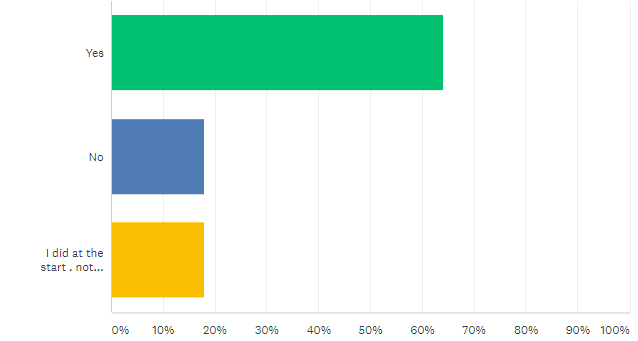
\includegraphics[width=1\textwidth]{img/Q1.png}
    \caption{Question 1 - Are you currently working during this pandemic?}
    \label{fig}
\end{figure}
\begin{figure}[h]
    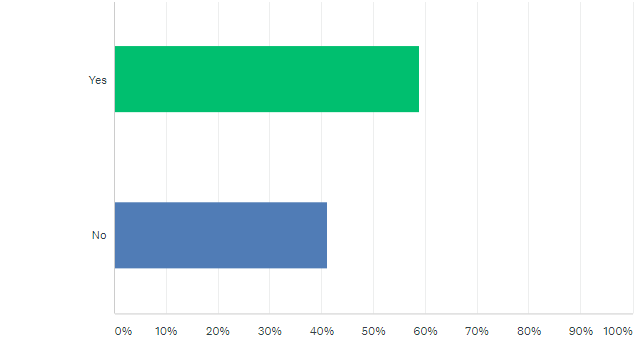
\includegraphics[width=1\textwidth]{img/Q2.png}
    \caption{Question 2 - In your workplace do all employees use the same clock-in machine?}
    \label{fig}
\end{figure}
\begin{figure}[h]
    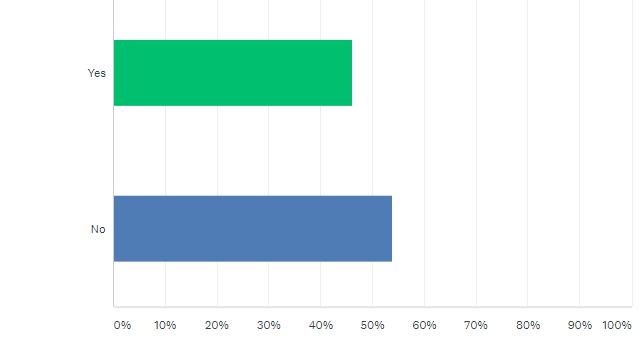
\includegraphics[width=1\textwidth]{img/Q3.png}
    \caption{Question 3 - If yes, does using the same machine as everyone else make you worried about covid-19 in the workplace and possibly catching it?}
    \label{fig}
\end{figure}
\begin{figure}[h]
    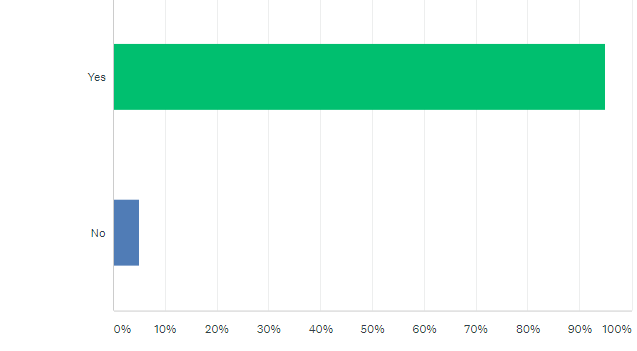
\includegraphics[width=1\textwidth]{img/Q4.png}
    \caption{Question 4 - Would you as an employee rather use a clock-in service which could be used via your personal smartphone and stop you and others touching the same surface thus reducing the risk of catching covid in the workplace?}
    \label{fig}
\end{figure}
\begin{figure}[h]
    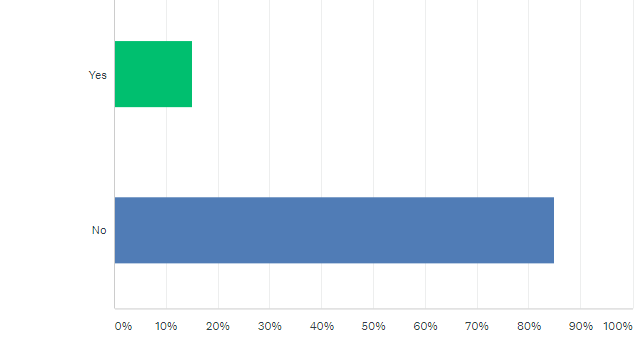
\includegraphics[width=1\textwidth]{img/Q5.png}
    \caption{Question 5 - Are you a business owner?}
    \label{fig}
\end{figure}
\begin{figure}[h]
    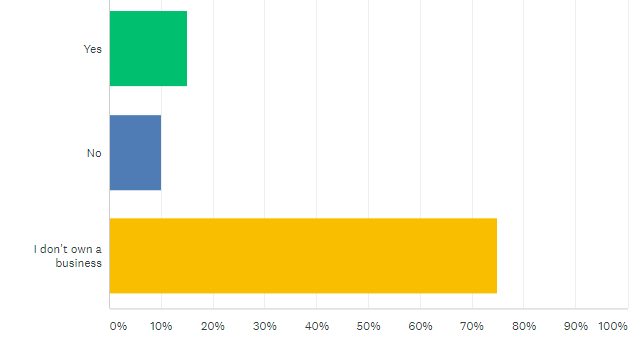
\includegraphics[width=1\textwidth]{img/Q6.png}
    \caption{Question 6 - If yes, would you be open to switching to a clock-in system which employees can access on their mobile phone which could help stop the spread of covid-19 in your workplace?}
    \label{fig}
\end{figure}
\begin{figure}[h]
    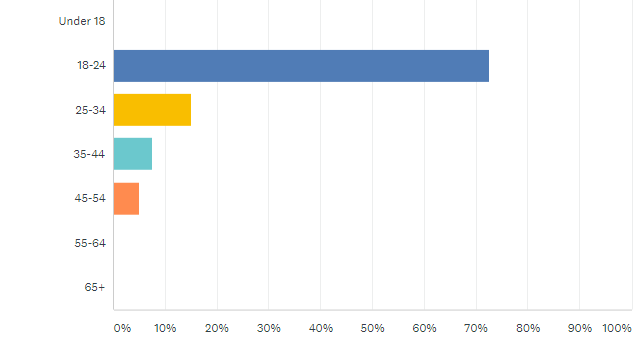
\includegraphics[width=1\textwidth]{img/Q7.png}
    \caption{Question 7 - What age group do you fall under?}
    \label{fig}
\end{figure}
\begin{figure}[h]
    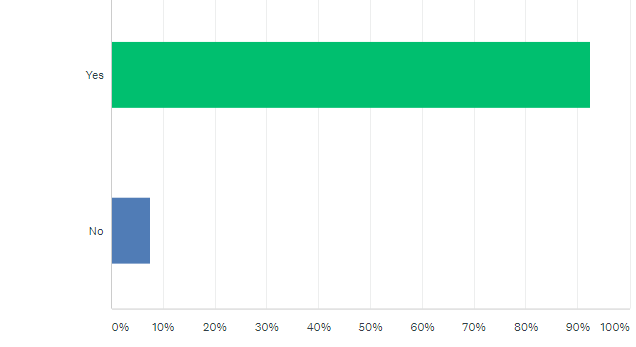
\includegraphics[width=1\textwidth]{img/Q8.png}
    \caption{Question 8 - Do you think a clock-in system like this is good in times like now and for future use even if you are not currently working?}
    \label{fig}
\end{figure}
\begin{figure}[h]
    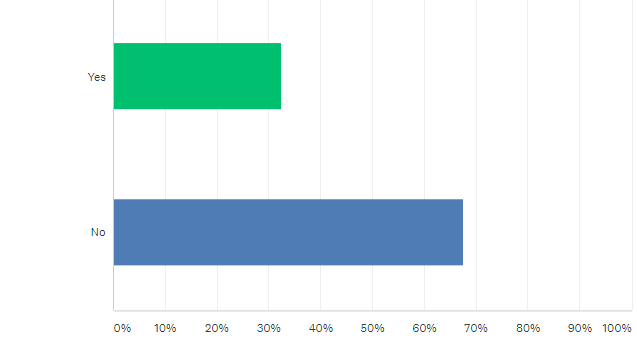
\includegraphics[width=1\textwidth]{img/Q9.png}
    \caption{Question 9 - If the application took a picture to verify your identity which could only be accessed by management would you have concerns with this?}
    \label{fig}
\end{figure}
\begin{figure}[h]
    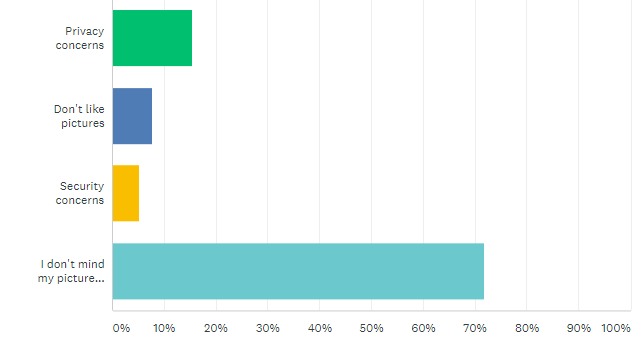
\includegraphics[width=1\textwidth]{img/Q10.png}
    \caption{Question 10 - If you have concerns about a photo being taken for clock-in purposes, why is this and would a text login option be acceptable?}
    \label{fig}
\end{figure}


\break
\break
The results and graphs showing the survey results can be found using the following link - https://www.surveymonkey.com/stories/SM-YZMFXF8C/
\\
\section{Clock-in Methods}
While working together as a team we did some research into different ways which employees could clock into the workplace. The main way we wanted to do was using Bluetooth beacons which, when an employee crossed a certain boundary, it clocked them in or out automatically. Obviously, down to the ongoing pandemic, it would have been a hard way to develop our application as with travel and meeting restrictions it would have meant that we as a team could not meet up in person to develop and test using the physical hardware we would need. If the pandemic was not on going this is the way we would have developed the application as we felt it offered a new and interesting dimension to development using code as in college we rarely, if ever, used our code on a hardware device other than a PC or laptop.
Due to these constraints, we changed our method of allowing employees to clock in and out. The method we decided on was a simple clock in and out button which appears once the user is logged in. Once pressed the details are pushed to our database and shows who is clocked in, what time they clocked in and what time they clocked out. We decided on this simple system as we believe it offers easy usability and simple navigation without being overly complicated. This will allow users to navigate and use the application with ease without a large learning curve while also providing all the functionality a manager will need by being able to see what time people clock in and out. A good article we found and used is located here \cite{appNeeds}. It offers great reasons as to why an application should be made simple and easy for the user.
\\
\section{Privacy}
When it comes to dealing with people’s personal information, it is important that privacy is put to the fore front of the research and planning as people need to know that their data is secure and who can view their sensitive material. As a team we have worked to reduce the amount of people able to view this data. Once the database is set up, that data should only be accessible by managers and owners of the business. This could possibly be done using a secure web application using a password or by having manager permissions set up on the application.
If data is unsecured it can lead to data breaches which can be extremely costly for businesses both financially and it can tarnish their reputation. Customers and employees should always know where their data goes and who can view it, why it’s needed by the company and who to contact if they have any concerns. From our survey it was clear to see some people don’t like their photograph being taken or used, so as a team we decided to allow a text login too which will help these people who don’t want their photo to be stored in a database.
\\
\section{Facial Recognition}
To allow people to clock in we decided to try and implement facial recognition. This would consist of the users account being set up with a photograph and then the application once opened would access their camera allowing the system to check if the person is registered and if they are grant them access to the application logged in as themselves. Facial recognition is something very new and we thought it was a great idea to include this. It offers a unique way to interact with the application from a user point of view. It also means that we do not have to store every picture every time someone clocks in. Using facial recognition will allow us to compare the face in the camera to the face we have set up for the user.
\\
As outlined above we have included facial recognition in this application as we as a team felt it was the most advanced form of identify verification we could develop. Along with this we thought it would be best that we try new and exciting features to broaden our knowledge base and help us become better developers by taking on features and subjects that would challenge us and make us must learn and research more. 
\\
Facial recognition will be used via the front facing camera of the customers phone to verify they are clocking in by comparing the image taken to an image stored on our database when their account was made. Facial recognition is relatively new and cutting edge, and we all agreed as a team that this would be a great key feature in our application. We also think that people will be more likely to use our application in the workplace if it’s as simple as a quick photo in the work place and then you are clocked in using your very own device.
\\

\section{Phones}
In this section we will talk about phones and how we as a team used them to incorporate our application idea which in turn helped us to solve the main problem we set out with. As you are probably aware, phones and mobile technology currently have essentially become another limb for many people. People will not leave the house without carrying a mobile phone nowadays. It was clear to us, as a team of developers looking to make a change, that phones would help play a key role in the development of this application.
\\
When developing an application there are many factors, we as a team must take into consideration before making any decisions some of which regard how many customers our application will be able to reach. As technology advances with huge technological breakthroughs being made on a regular basis, it comes as no surprise that the phone market can be a bit scattered with some people using iPhone 6’s for example and others using the new latest Samsung S21. The clear difference in the technology in older and new phones meant that we had to try and develop an application that would run comfortably on both.
\\
\subsection{Phone users}
According to research carried out by Irish Life \cite{smartPhoneUsage} 90 per cent of Irish adults owned a smartphone. The top three uses phone by people surveyed were checking emails, checking social media platforms and checking the news and weather. As a development team this was a clear indication that our idea to have people clock into work using their own device was more than achievable. In Ireland in 2020 \cite{Statista}, Statista published that there was 3.62 million smartphone users in Ireland and in 2021 3.68 million smartphone users. This will result in most people being able to download our app and login that way. From our research we found that Android has 45.39 percent of the  Mobile Vendor Market Share in Ireland which we feel is significant \cite{Mobile}. However, if an employee did not have a smartphone, the company should provide an Android tablet to allow the employee to clock in.
\\
\subsection{Phone Cameras and Different Phones}
Firstly, regarding phones in the development side of our application we had to consider the camera quality which people had on their phone. Newer phones on the market such as the iPhone 11 \cite{iPhone11} have a front facing camera with 12 megapixels (MP) whereas slightly older models like the iPhone 6 only have a front camera with 1.2 megapixels \cite{iPhone6} (MP). As evident by the specifications outlined above, older models would possibly struggle with uploading a clear picture that the facial recognition could use for a login. To combat this, we as a team felt we could solve two problems with one solution. As seen in our survey, and in today’s world in general, some people do not like their photos being taken, especially by technology companies who may store them. We as a team decided to include a text login option which would be a solution to people not wanting a photo being taken and for people who might not have a strong enough camera. We felt it unreasonable to cut out some people and have no option for them other to buy a new phone especially when this is a workplace feature.
\\
We have developed our application and tried to accommodate most phone sizes to be compatible with our application. One of the short falls of using a completely new language and development environment for us was we were not used to android studio whatsoever and we have not used any platform similar in our time as developers. One of Android Studios many short fallings, which we will discuss later in this document, is that it can be extremely clunky and unhelpful to developers. In order to get the application working on different sized devices Android Studio does not offer auto scaling like other platforms and instead relies on the developer to implement separates pages which can be run on separate mobile devices. This alone is extremely frustrating to us as developers, as it creates a lot of extra work and time but also makes our work space and file system look like a complete mess and easily leads to getting lost in the endless amounts of pages you have to scavenge through in order to change something, not to mention the fact it has to be changed on every page individually.
\\

\chapter{Frameworks}
\section{Kotlin}
We decided to work with the programming language Kotlin \cite{kotlin} for our final year project as it was best suited to developing our application. The Kotlin programming language was the most suited to making an Android App when comparing it to other possible languages that we could use. It also helped when we discovered that Google had said that Kotlin was the preferred language for Android App developers as it showed that the majority of app developers trusted this language to use on their application which cleared any doubts that we had about using this programming language.
\\
\\
 Even though we were unfamiliar with using this language before during our time in the course, we were excited about the prospect of working with a new language and it would also benefit us that we were learning something new and different from before and also that it was one that we could trust to get our application done to the best of our ability. We wanted to challenge ourselves as well with doing another language as we have been used to doing other languages for a period of time before undergoing assignments and we wanted to start off with Kotlin by learning it while doing our final year project as a practice tool for us working with other languages in the future.
 \\
 \\
This language was unveiled in 2011 as a new language for the Java Virtual Machine alongside Java which was the main and most worked with language for android apps at that time. Where this language differs to Java is that it does not have its own built system or package manager as open source tools such as Gradle and Maven.
\\
\\
We worked on Kotlin on Android Studio which is the official integrated development environment (IDE) for Google’s Android System. We had to install a plugin for using Kotlin on our Android Studio in order for it to work. All the IDE features worked perfectly with Kotlin. So good that you could work on an application using both Kotlin and Java on the same project and it would still come out well. The advantage that Kotlin has over Java in terms of code is there are less lines of code to be written in Kotlin to complete feature for the application as opposed to many lines of code that has to be written in Java just to complete a method.
\\
\\
This language like any other language has not been the easiest to start off with but once we got our heads wrapped around with, we found it much easier to work with it.
\\
\section{Android Studio}
Android Studio is the official integrated development environment (IDE) for Google’s Android System \cite{androidStudio}. This is designed for Android development specifically. It is used for working on code when developing an application usually using the Kotlin programming language and also other languages such as Java.
\\
\\
Android Studio let’s us users change our code and push it without having to restart the app or even the current activity that we would be working on. The code editor in Android Studio is impressive as well, as solutions would come up if you wanted to include a certain method or statement and you are able to press the tab button in order to insert the code automatically into the page that’s being worked on.
\\
\\
When working with Android Studio in regards to launching the compiled code, we would use an emulator to launch the code that we worked on or we could run it on our own smart devices by connecting it with a USB (Universal Serial Bus) cable. The role of the emulator is that the purpose of it is to run a totally different software system in the software system that they’re already on so for example, running a mobile application on Android Studio. In terms of running our app with using our own smart devices, we have to be able to enable USB Debugging on the developer options feature in the settings of a smart device \cite{usbDebugging}. Then the user will be able to launch their app on their own smart devices.
\\
\section{MongoDB}
MongoDB is the database that we are using as the database for our final year project. The purpose of this database application that it stores data in a JSON like document \cite{MongoDBAtlas}. This database is able to store the information of details that a user has entered about themselves. For example, if you were entering an address, it would start off with either an ID or the name of the person and would then enter the address and possibly their phone number as well and then it is saved on the database. Then you could use a sort order for the people who logged in first, for example having the people who logged in the earliest compared to the ones who logged in later on. This is one of the most popular databases that are used for websites and we have experience already with using this before with our React app project that we did last year. We are also using React as well for our code as well on Visual Studio Code. It is a front end, JavaScript library used for building user interfaces \cite{react}. It is very useful that we have worked with react already, so it will be easier to work with this time around and it will also help with our website as well.
\\
\\
What we’re exactly using this is for storing the information of the time when the employees in the workplace will be clocking in and out of their workplace so that the manager will be able to see if the employees will be coming into work on time. It will consist with having the username or name of the person being entered into the app in order for them to login and clock in and then be able to take a picture of themselves then as a form of saying they have signed themselves into the workplace. The exact details of when exactly the employee logged into the workplace should come into the database, with their name and email being shown on the database while also the exact time they clocked into work and when they clocked out as well from work. We will also try and have the facial recognition system to be able to recognise the person that is taking the photo of themselves as an easier way for them to be able to clock into the app then after their face has been recognised.
\\
\section{Website and App}
As opposed to making our website, we will be using MongoDB Atlas as our database so we will be able to see who will be clocking in and clocking out from the website. We will first have to connect the website to the database in order for there to be a connection established. For the coding part of the website, we are using the Visual Studio Code Application as it is the best one for working with websites that collaborate with MongoDB Atlas. 
\\
\\
Visual Studio Code was the same application that we used last year in the Data Representation and Querying module with Martin Kenirons. In that module we had to create an application using React where we used MongoDB Atlas as our database and we used visual studio code to write up the coding part of our app. Then we are able to launch the application from the command line using the npm start command and the localhost server will launch on your browser.
\\
We feel that the MongoDB Atlas is the perfect database to work on as we already have experience working with it from before and it is highly recommended by other sources as well as one of the best databases to work on in terms of making websites and having the exact details of every feature that’s pushed and saved to the database.
\\
\\
For the mobile app part of our final year project, we are using MongoDB Realm. Mongo DB Realm is basically the cloud synchronization piece that connects a MongoDB Atlas database to a client side realm data \cite{MongoDBRealm}. To have this work with our MongoDB Atlas, we use realm sync to create a synced realm that partitions our MongoDB Realm database into a local realm and syncs data between the database and all clients who use it. This is one of the most popular mobile databases used by mobile developers, as over one hundred thousand of them worldwide have used them and it is perfect for us to use for our mobile application as we are already using MongoDB Atlas for our website.
\\
\section{Confluence and Jira}
Jira is a software that is used for software teams to plan track and release software \cite{jira}. Jira was suggested to us by our supervisor. Jira was very beneficial for us to use as it let us create user stories, plan sprints and distribute tasks for our team. Jira was very beneficial for keeping track of our work so we could easily plan out the project. In Jira we had sprints where we would plan out a sprint. We found by doing sprints it let us get work completed very efficiently.
\\
Confluence is a collaborative work space where we could all input into and was used for our milestones, gantt chart, user stories and project architecture \cite{confluence}. We included a milestones chart and a gantt chart which was a really useful visual aid as it meant that we had to work towards a deadline which made it easier.
Another feature we used in confluence was user stories. "A user story is an informal, general explanation of a software feature written from the perspective of the end user. Its purpose is to articulate how a software feature will provide value to the customer." \cite{UserStory} We decided to include a table on our page which included User Story Title which describes the title of the user story, User Story Description which was a brief description of our user story and what it entails, Importance which was level of importance and Notes where we could add notes onto it to the user story. Some of the User stories we included were Location feature, Facial Recognition Feature, Sickness Feature, Access Information, Database, Privacy, Clock-In Feature, Break Feature and Clock-Out Feature. \\
\begin{figure}
    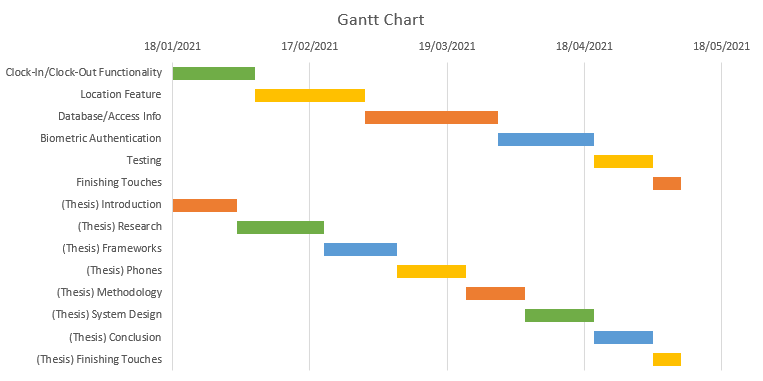
\includegraphics[width=1\textwidth]{img/Gantt_Chart.png}
    \caption{Gantt Chart done in confluence}
    \label{fig}
\end{figure}

\section{Frameworks that were not used for FYP}
Some of the frameworks that we considered using for our final year project (FYP), but we decided against it included the likes of Xamarin and Firebase. We had worked with Xamarin before in the Mobile App module in second year and Firebase in the Professional Skills in IT module in third year. We had enjoyed working with those frameworks at that time but with it being our final year project and all, we thought it would be great if we challenged ourselves as students and learn a new language in Kotlin as it would feel more rewarding to us if we got it done knowing that we done it from the start ourselves.
\\
\\
We briefly had considered Firebase as a database that we could use for our application. We had used it before on a React project that we done last year. So we already had a good bit of experience with working with Firebase, especially with the login section where we could have used something similar for our application to put our emails and password in where it could be saved then in the database. However we had read from a few sources to how good MongoDB integrates as a database with other applications and how it was highly rated as one of the best databases for websites and apps. It was also a plus that we had used it before so it was an obvious choice to use it again.
\\
\\
Even though these would all have been great frameworks to use, we are all satisfied with the choices that we made and we feel that we are learning while working at the same time.
\\
\\

\chapter{Methodology}
\section{Overview}
In this section, we will describe and review the approach that we took in developing of
this project, we will describe the methodology used why it was necessary, how it was
implemented and how it helped the development of the application progress overall.
After reading this section, the reader should have a clear understanding of the complexity
and scale of the project as well as the steps taken throughout the development. The project
design was not fully completed and features were not finalized therefore we needed to use
a system that would help us keep on top of any changes and where issues could be dealt
with in an easy and efficient manner.
After researching many methodologies such as the Waterfall and Lean we had decided that the best methodology for our project was Scrum which is an agile project
management methodology or framework. Agile methodology is a way of continuous iteration of both developing and testing \cite{agile}. Unlike the Waterfall methodology which was an
option for us to use both development and testing of the project are concurrent. There
are many benefits of using this methodology and here are some of the ones that helped us determine that this was the right decision.
Agile allows the team to effectively prioritize features and workings and also big changes to
the project can be implemented even towards the end of the development. The agile methodology was a perfect way to help us with the development but we were not able to utilize all of its features such as the daily scrum meetings so we instead had a team meeting once a week discussing the work completed and forward approach. We attended meetings with our supervisors as often as possible informing them of the progress
and gathering their thoughts on the progress as well as the necessary future development.

\subsection{Using Agile} 
Within the agile Software Development Life Cycle, work is divided into sprints, with the goal of producing a working product at the end of each sprint. A sprint typically lasts two weeks, or 10 business days. The workflow of a sprint should follow this basic outline:
\\
\\
\textbf{Plan}: The sprint begins with a sprint planning meeting, where we had a meeting where we layed out components for the upcoming week of work. Once we were happy with this we then prioritised the work and assigned a task to each team member.
\\
\\
\textbf{Develop}: Design and develop what needs to be done to complete the task.
\\
\\
\textbf{Test/QA}: Complete thorough testing and documentation of results before delivering it to team members.
\\
\\
\textbf{Deliver}: Present the working product or software to team members and to our supervisor.
\\
\\
\textbf{Assess}: Gather Feedback from the team and from the supervisor and make changes accordingly.
\\
\\
\textbf{Sprint Planning}:
The team and supervisor discuss the top priority user stories and determine which ones will be implemented in the next sprint
\\
\\
\textbf{Sprint Backlog}: Is the list of the user stories which are committed for the next sprint.
\\
\\
\textbf{Sprint}:
This is a one to three week time frame where the user stories in the sprint backlog are developed by the team. During the sprint meetings its a team meeting where each team member discussed the completed work, the part each person is working on and if anyone needs help or has ran into issues in the work they were doing.
\\

\section{Sprint 1}
\subsection{Clock In/Out, Break, Sickness Feature}
\subsubsection{Description}
For our first sprint, we decided to work on the front end of the app. This involved how the app looked, how easy it was to use, and allowing the employee to be able to navigate through the app. So he/she could clock in, go on break, clock out, and notify the manager if they are feeling unwell. To start this sprint research was the first item that we wanted to cover. We started off by making a basic android application while we were discussing what pages to do. The language we decided to use for the application was Kotlin, which was going to be coded using Android Studio. As this was a new language, our first goal was to make sure everyone had a similar understanding of the language. For storage, we decided to use MongoDB, as we had some previous experience with the database in the past. So at this stage it meant that we had a solid base to the project that we could build on easily and the team were all on the same page.
\subsubsection{Allocation}
Daniel was allocated to lead this sprint.
\subsubsection{Frameworks, Technologies and Languages}
Kotlin, Android Studio, XML
\subsubsection{Code Snippets}
The below code shows some of the code used for the clock in activity. The code shows the application getting the current time. The application then gets the clock in times already stored on our database in MongoDB. After this it either adds the users time to the database if it is their first time using the application and if not it simply updates the users time stored in the database.
\begin{lstlisting}[caption={Clock In code}, label={lst:example1}, language=Kotlin]
// Push clock in to mongodb when employee clocks in,
// and update isclockedin to true
@RequiresApi(Build.VERSION_CODES.O)
private fun clockIn(){
    // Get current time
    val currentClockInTime = LocalTime.now()

    // Find clockintimes collection on mongodb
    val user = realmApp.currentUser()
    val mongoClient =
            user!!.getMongoClient("mongodb-atlas") // service for MongoDB Atlas cluster containing custom user data
    val mongoDatabase =
            mongoClient.getDatabase("tracker")
    val mongoCollectionClockInTimes =
            mongoDatabase.getCollection("clockintimes")

    // Find document in collection with user's ID
    val queryOne = Document("_partition", "user="+user.id)
    // Update document with the current time
    val updateClockInTimes = Document("_partition", "user="+user.id)
            .append("clockedInTime", currentClockInTime.format
            (DateTimeFormatter.ofLocalizedTime(FormatStyle.MEDIUM)))
            .append("name", user?.customData?.get("name"))
    // Allow upsert (if document not found, create one)
    val updateOptions = UpdateOptions().upsert(true)
    // Update/upsert document
    mongoCollectionClockInTimes?.updateOne(queryOne, updateClockInTimes, updateOptions)?.getAsync { task ->
        if (task.isSuccess) {
            if(task.get().upsertedId != null){
                Log.v("EXAMPLE", "upserted document")
            } else {
                Log.v("EXAMPLE", "updated document")
            }
        } else {
            Log.e("EXAMPLE", "failed to update document with: ${task.error}")
        }
    }

    // Find isclockedin collection on mongodb
    val mongoCollectionIsClockedIn =
            mongoDatabase.getCollection("isclockedin")

    // Find document in collection with user's ID
    val queryTwo = Document("_partition", "user="+user.id)
    // Update document with the current time
    val updateIsClockedIn = Document("_partition", "user="+user.id).append("clockedIn", true)
    // Update/upsert document
    mongoCollectionIsClockedIn?.updateOne(queryTwo, updateIsClockedIn, updateOptions)?.getAsync { task ->
        if (task.isSuccess) {
            if(task.get().upsertedId != null){
                Log.v("EXAMPLE", "upserted document")
            } else {
                Log.v("EXAMPLE", "updated document")
            }
        } else {
            Log.e("EXAMPLE", "failed to update document with: ${task.error}")
        }
    }
}
\end{lstlisting}


The below code is much the same as above. It shows the clock out activity used by us in android studio. Again the application gets the current time then checks our database for the user and their old time. If the user exists on the database already their clock out time is changed and if not they are simply added to the database and it saves the data to the database.
\begin{lstlisting}[caption={Clock Out code}, label={lst:example1}, language=Kotlin]
// Push clock out time to mongodb when employee clocks out,
// and update isclockedin to false
@RequiresApi(Build.VERSION_CODES.O)
private fun clockOut(){
    // Get current time
    val currentClockOutTime = LocalTime.now()

    // Find clockouttimes collection on mongodb
    val user = realmApp.currentUser()
    val mongoClient =
            user!!.getMongoClient("mongodb-atlas") // service for MongoDB Atlas cluster containing custom user data
    val mongoDatabase =
            mongoClient.getDatabase("tracker")
    val mongoCollection =
            mongoDatabase.getCollection("clockouttimes")

    // Find document in collection with user's ID
    val query = Document("_partition", "user="+user.id)
    // Update document with the current time
    val update = Document("_partition", "user="+user.id).append("clockedOutTime", currentClockOutTime.format(DateTimeFormatter.ofLocalizedTime(FormatStyle.MEDIUM)))
            .append("name", user?.customData?.get("name"))
    // Allow upsert (if document not found, create one)
    val updateOptions = UpdateOptions().upsert(true)
    // Update/upsert document
    mongoCollection?.updateOne(query, update, updateOptions)?.getAsync { task ->
        if (task.isSuccess) {
            if(task.get().upsertedId != null){
                Log.v("EXAMPLE", "upserted document")
            } else {
                Log.v("EXAMPLE", "updated document")
            }
        } else {
            Log.e("EXAMPLE", "failed to update document with: ${task.error}")
        }
    }

    // Find isclockedin collection on mongodb
    val mongoCollectionIsClockedIn =
            mongoDatabase.getCollection("isclockedin")

    // Find document in collection with user's ID
    val queryTwo = Document("_partition", "user="+user.id)
    // Update document with the current time
    val updateIsClockedIn = Document("_partition", "user="+user.id).append("clockedIn", false)
    // Update/upsert document
    mongoCollectionIsClockedIn?.updateOne(queryTwo, updateIsClockedIn, updateOptions)?.getAsync { task ->
        if (task.isSuccess) {
            if(task.get().upsertedId != null){
                Log.v("EXAMPLE", "upserted document")
            } else {
                Log.v("EXAMPLE", "updated document")
            }
        } else {
            Log.e("EXAMPLE", "failed to update document with: ${task.error}")
        }
    }
}
\end{lstlisting}

\section{Sprint 2}
\subsection{Location Feature}
\subsubsection{Description}
In our second sprint, we started on the location feature. This involved allowing the app to check if the employee was at the workplace, via their smartphone location. If the employee is at the workplace, the clock in button would be enabled, otherwise, it would be disabled, and the employee would be unable to clock in. This worked by setting the latitude and longitude of the workplace in Android Studio and then checking if the employees current latitude and longitude was equal to it. We rounded the workplaces latitude and longitude to .3 decimal places so not all employees would have to go to the same area of the workplace to clock in.
\subsubsection{Allocation}
Jack was allocated to lead this sprint.
\subsubsection{Frameworks, Technologies and Languages}
Kotlin, Android Studio, Android Location Provider
\subsubsection{Code Snippets}
The above screenshot shows how the location feature code works. It gets the clients location using FusedLocationProviderClient. It uses the employees current location and checks it against the location stored on the database as the workplace and if the person is not in this area they are unable to clock into their workplace.
\begin{lstlisting}[caption={Location code}, label={lst:example1}, language=Kotlin]
// https://www.tutorialspoint.com/how-to-track-the-current-location-latitude-and-longitude-in-an-android-device-using-kotlin
// Finds the location of the employee using the FusedLocationProviderClient
private fun getLastLocation() {
    // Check permission
    if (ActivityCompat.checkSelfPermission(
                    this,
                    Manifest.permission.ACCESS_FINE_LOCATION
            ) != PackageManager.PERMISSION_GRANTED && ActivityCompat.checkSelfPermission(
                    this,
                    Manifest.permission.ACCESS_COARSE_LOCATION
            ) != PackageManager.PERMISSION_GRANTED
    ) {
        return
    }

    fusedLocationClient?.lastLocation!!.addOnCompleteListener(this) { task ->
        if (task.isSuccessful && task.result != null) {
            lastLocation = task.result

            // employees current location
            val latLocation = (lastLocation)!!.latitude.round(3)
            val longLocation = (lastLocation)!!.longitude.round(3)

            // Output employee location details to console
            Log.v("EXAMPLE", "employee latitude: $latLocation")
            Log.v("EXAMPLE", "employee longitude: $longLocation")

            // Find location collection on mongodb
            val user = realmApp.currentUser()
            val mongoClient =
                    user!!.getMongoClient("mongodb-atlas") // service for MongoDB Atlas cluster containing custom user data
            val mongoDatabase =
                    mongoClient.getDatabase("tracker")
            val mongoCollection =
                    mongoDatabase.getCollection("location")

            // Find first document in collection
            val query = Document()
            mongoCollection?.findOne(query)?.getAsync { task ->
                if (task.isSuccess) {
                    // Latitude and Longitude in document
                    val latitude = task.get()["latitude"]
                    val longitude = task.get()["longitude"]
                    // Output location details in document to console
                    Log.v("EXAMPLE", "successfully found latitude: $latitude")
                    Log.v("EXAMPLE", "successfully found longitude: $longitude")

                    // Enable button if employee location is equal to latitude & longitude in document
                    if(latLocation == latitude && longLocation == longitude){
                        button_clockin.isEnabled
                    }
                    else{
                        Toast.makeText(baseContext, "Your location is not in the workplace, please close app and try again", Toast.LENGTH_LONG).show()
                    }
                } else {
                    Log.e("EXAMPLE", "failed to find document with: ${task.error}")
                }
            }
        } else {
            Log.w(TAG, "getLastLocation:exception", task.exception)
            showMessage("No location detected. Make sure location is enabled on the device.")

            // Disable clock in button if location is not turned on
            button_clockin.isEnabled = false
        }
    }
}
\end{lstlisting}

\section{Sprint 3}
\subsection{Database/Access Info Feature}
\subsubsection{Description}
This sprint involved working on the back-end of our application and allowing the manager to be able to easily access the info stored on the database. To do so, we used MongoDB as we have had prior experience with the database program, and it is also document-oriented, which is suitable for our need to store the employees’ clock in/out times.
Firstly, we worked on allowing the employees to log in to the app. For the employee to log in however, the manager first must create an account for the employee. When the manager had done so, the employee could then log in with their details, which are an email and password, and then reset their password in the app. The manager can also edit the details of their employees, such as their first name, last name, date of birth, and emergency contact.
We then started on pushing the clock in and out times to MongoDB. So, the manager could view the time an employee clocked in, the current time of when the employee presses the clock in button is pushed to a MongoDB collection. The same is done for when an employee clocks out.
Following this, we worked on a clocked in collection that tracks whether an employee is clocked in or not. This was done to improve the user experience of the app, so that if an employee closes the app after pressing the clock in button, he/she would be brought to the clocked in page when reopening the app. 
We also worked on allowing the manager to change the latitude and longitude of the workplace, via the app, to further enhance the location feature.
As we felt all the needed details were being pushed to the database, we started on creating the website. This website allows the manager to view the times that employees clocked in, clocked out, and their details. To also ensure the privacy of the employee details, the manager has to log in to the website via a Heroku add-on, wwwhisper \cite{wwwhisper}. This add-on is configured so that only the managers email can be used to log in, and when he/she logs in, they are sent a unique code, via email, that they have to enter to access the website.
\subsubsection{Allocation}
Ryan was allocated to lead this sprint.
\subsubsection{Frameworks, Technologies and Languages}
Kotlin, Android Studio, MongoDB, MERN, Heroku, Visual Studio Code
\subsubsection{Code Snippets}
\begin{figure}[h]
    \centering
    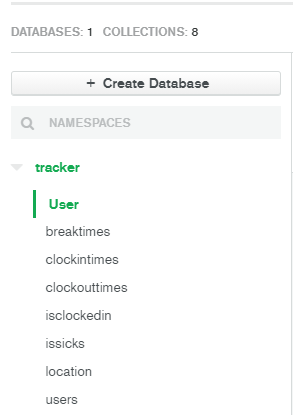
\includegraphics[width=0.4\textwidth]{img/database.png}
    \caption{MongoDB}
    \label{fig}
\end{figure}
The above image shows our MongoDB and the tables it contains. MongoDB is where our application send all the information we need for the application to work such as employee details, clock times and locations. What is stored in each section is very self-explanatory such as location storing locations and users storing our users of the application.
\section{Sprint 4}
\subsection{Biometric Authentication Feature}
\subsubsection{Description}
To further improve the user experience and secure their account, we decided to add biometric authentication \cite{bioauth} to our app. This allows the employee to log in by using their stored biometrics, depending on which type of biometric they have stored. These biometrics can include fingerprint, eye, and face. For example, if they have their fingerprint stored on their smartphone, the employee can log in by using their fingerprint. To accomplish this, we took advantage of the SharedPreferences on Android to store the employees’ email and password, whilst encrypting the password in the process. This process works by the employee clicking enable biometric authentication on the log in page, entering their email and password to be stored and encrypted. From then on, the employee can log in to the app via biometric authentication.  
\subsubsection{Allocation}
Shane was allocated to lead this sprint.
\subsubsection{Frameworks, Technologies and Languages}
Kotlin, Android Studio, Android Biometrics
\subsubsection{Code Snippets}
Once enabled an employee simply has to add their login email and password. When this is active it encrypts the password and saves it so that it can easily be retrieved by the application. Once the employee opens the app again they will have the option to log in via biometric authentication. Scanning their fingerprint will then retrieve this password, decrypt it and log the employee in, leading to much faster login times.
\begin{lstlisting}[caption={Biometric Authentication code}, label={lst:example1}, language=Kotlin]
private fun showBiometricPromptForEncryption() {
    val canAuthenticate = BiometricManager.from(applicationContext).canAuthenticate()
    if (canAuthenticate == BiometricManager.BIOMETRIC_SUCCESS) {
        val secretKeyName = getString(R.string.secret_key_name)
        cryptographyManager = CryptographyManager()
        val cipher = cryptographyManager.getInitializedCipherForEncryption(secretKeyName)
        val biometricPrompt =
            BiometricPromptUtils.createBiometricPrompt(this, ::encryptAndStorePassword)
        val promptInfo = BiometricPromptUtils.createPromptInfo(this)
        biometricPrompt.authenticate(promptInfo, BiometricPrompt.CryptoObject(cipher))

    }
}

private fun encryptAndStorePassword(authResult: BiometricPrompt.AuthenticationResult) {
    authResult.cryptoObject?.cipher?.apply {
        UserCredentials.password?.let { token ->
            Log.d(TAG, "The token from server is $token")
            val encryptedServerTokenWrapper = cryptographyManager.encryptPassword(token, this)
            cryptographyManager.persistCiphertextWrapperToSharedPrefs(
                    encryptedServerTokenWrapper,
                    applicationContext,
                    "biometric_prefs",
                    Context.MODE_PRIVATE,
                    "ciphertext_wrapper"
            )
        }
    }
    onLoginSuccess("Successfully enabled biometric authentication!")
}
\end{lstlisting}

\section{Sprint 5}
\label{sec:Testing}
\subsection{Testing}
\subsubsection{Description}  
For testing our app, we decided to use a combination of unit testing and instrumentation testing. Unit testing consists of testing the logic of the app and the features of the app individually \cite{unittest}. For example, if the email and password the employee uses to log in to the app is valid. Instrumentation testing involves testing the behaviour of the app across different devices by running the tests on physical devices and emulators \cite{instrumentationtest}. For example, the user experience of the app may change when deployed on different smartphones, in regards to the layout of images or text on pages, loading times, and app performance.
\\

For unit testing, we tested the following features of the app:
\begin{itemize}
    \item \textbf{Logging in/out}  
    \begin{center}
     \begin{tabular}{||c c c||} 
      \hline
      Test & Expected Output & Pass/Fail \\ [0.5ex] 
      \hline\hline
      Log in & Log in successful & Pass \\
      \hline
      Log out & Log out successful & Pass \\
      \hline
      Biometric & User can log in with their  & Pass \\
      Authentication & biometric credentials &  \\
      \hline
     \end{tabular}
    \end{center}
    \item \textbf{Clocking in/out}
    \begin{center}
     \begin{tabular}{||c c c||} 
      \hline
      Test & Expected Output & Pass/Fail \\ [0.5ex] 
      \hline\hline
       Clock in & Employee clocks in and is & Pass \\
        & brought to clock out page &   \\
      \hline
      Clock out & Employee clocks out and is & Pass \\
        & brought back to clock in page &   \\
      \hline
      Clocked in & Employee brought to clock out page & Pass \\
        & if already clocked in &   \\
      \hline
     \end{tabular}
    \end{center}
    \item \textbf{Going on/starting/finishing break}
    \begin{center}
     \begin{tabular}{||c c c||} 
      \hline
      Test & Expected Output & Pass/Fail \\ [0.5ex] 
      \hline\hline
      Break & Employee brought to break page & Pass \\
      \hline
      Start Break & Employee starts their break & Pass \\
      \hline
      End Break & Employee finishes their break and is & Pass \\
        & brought back to clock out page &   \\
      \hline
     \end{tabular}
    \end{center}
    \item \textbf{Notifying manager if sick}
    \begin{center}
     \begin{tabular}{||c c c||} 
      \hline
      Test & Expected Output & Pass/Fail \\ [0.5ex] 
      \hline\hline
      Employee is sick & Manager is notified & Pass \\
      \hline
      Employee is not sick & Manager isn't notified & Pass \\
      \hline
     \end{tabular}
    \end{center}
    \item \textbf{Resetting password}
    \begin{center}
     \begin{tabular}{||c c c||} 
      \hline
      Test & Expected Output & Pass/Fail \\ [0.5ex] 
      \hline\hline
      Reset Password & Employee can reset their password & Pass \\
      \hline
     \end{tabular}
    \end{center}
    \item \textbf{Adding/editing employees' details}
    \begin{center}
     \begin{tabular}{||c c c||} 
      \hline
      Test & Expected Output & Pass/Fail \\ [0.5ex] 
      \hline\hline
      Add employee & Manager can add an employee & Pass \\
        & to the app &   \\
      \hline
      Edit employee details & Manager can edit an employees details & Pass \\
       & (Name, D.o.B, Emergency Contact &  \\
      \hline
     \end{tabular}
    \end{center}
    \item \textbf{Changing the location of the workplace}
    \begin{center}
     \begin{tabular}{||c c c||} 
      \hline
      Test & Expected Output & Pass/Fail \\ [0.5ex] 
      \hline\hline
      Change location & Manager can change the location & Pass \\
        & of the workplace &   \\
      \hline
     \end{tabular}
    \end{center}
\end{itemize}


For instrumentation testing we used Robo Test \cite{robotest}, a testing tool that is integrated with Firebase Test Lab \cite{firebasetestlab}. Robo Test works by taking in input from Android Studio, such as an accepted email and password, to navigate through the app and simulate user activities. Robo Test also takes a video of what the Robo done whilst going through the app and provides logs on what activities passed and failed. Through using Firebase Test Lab, we could test our app on multiple devices and configurations, to see if our app runs successfully on many different smartphones. 
\\
Links for recorded videos of RoboTest:
\begin{itemize}
    \item Employee test: \url{https://www.youtube.com/watch?v=XD979nVJcLo}
    \item Manager test: \url{https://www.youtube.com/watch?v=tih0fi2N0zg}
\end{itemize}

For testing the website, we decided to use unit testing. To do so, we tested the following features:
\\

\begin{itemize}
    \item \textbf{Logging in}
    \begin{center}
     \begin{tabular}{||c c c||} 
      \hline
      Test & Expected Output & Pass/Fail \\ [0.5ex] 
      \hline\hline
      Log in & Manager is sent an email & Pass \\
       & and can log in with code &  \\
      \hline
     \end{tabular}
    \end{center}
    \item \textbf{Clocking in times}
    \begin{center}
     \begin{tabular}{||c c c||} 
      \hline
      Test & Expected Output & Pass/Fail \\ [0.5ex] 
      \hline\hline
       Clock in times & Employee clock in times displayed & Pass \\
      \hline
     \end{tabular}
    \end{center}
    \item \textbf{Clocking out times}
    \begin{center}
     \begin{tabular}{||c c c||} 
      \hline
      Test & Expected Output & Pass/Fail \\ [0.5ex] 
      \hline\hline
       Clock out times & Employee clock out times displayed & Pass \\
      \hline
     \end{tabular}
    \end{center}
    \item \textbf{Break times}
    \begin{center}
     \begin{tabular}{||c c c||} 
      \hline
      Test & Expected Output & Pass/Fail \\ [0.5ex] 
      \hline\hline
      Break times & Employee break times displayed & Pass \\
      \hline
     \end{tabular}
    \end{center}
    \item \textbf{Sick Employees}
    \begin{center}
     \begin{tabular}{||c c c||} 
      \hline
      Test & Expected Output & Pass/Fail \\ [0.5ex] 
      \hline\hline
       Employee sick list & Employees unable to make work  & Pass \\
         & displayed here  &   \\
      \hline
     \end{tabular}
    \end{center}
    \item \textbf{Employees' details}
    \begin{center}
     \begin{tabular}{||c c c||} 
      \hline
      Test & Expected Output & Pass/Fail \\ [0.5ex] 
      \hline\hline
      Employee details & Employee details displayed & Pass \\
      \hline
     \end{tabular}
    \end{center}
    \item \textbf{Remove details}
    \begin{center}
     \begin{tabular}{||c c c||} 
      \hline
      Test & Expected Output & Pass/Fail \\ [0.5ex] 
      \hline\hline
      Remove details & Manager can remove details & Pass \\
      \hline
     \end{tabular}
    \end{center}
\end{itemize}

\subsubsection{Allocation}
Jack was allocated to lead this sprint.
\subsubsection{Frameworks, Technologies and Languages}
Kotlin, Android Studio, Firebase Test Lab, MERN, Visual Studio Code
\subsubsection{Code Snippets}
\begin{figure}[h]
    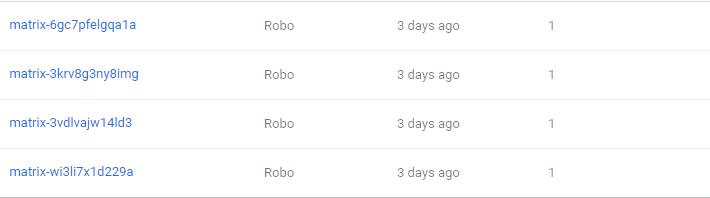
\includegraphics[width=1\textwidth]{img/testingCode.png}
    \caption{Application Testing}
    \label{fig}
    The above screenshot shows our testing carried out using Test Lab on Firebase. This is a really handy testing platform and allowed us to test efficiently and quickly using the robo tests feature. In the screenshot you firsty see the test case name followed by the type and when it was last run. Each test case ran on the application tested a different feature and we have included the videos of these tests being run and passing above this where we discuss our sprints.
\end{figure}
\section{Project Dissertation Allocation}
The project dissertation was completed with the four members of our team working together at once on development or breaking into groups and taking on specific tasks that required development. We had meetings at least 4 times as week with each other where we discussed the various areas that needed development, how we were handling our work and where we could improve our application which helped immensely with our work load , group dynamics and definitely helped us manager our time and development as best we could considering we had a large workload with other modules in college at the same time as developing this project.
We feel that the write up was divided fairly and evenly with each one of us working on
comparable amounts of this document.


\chapter{System Design}
\begin{figure}[h]
    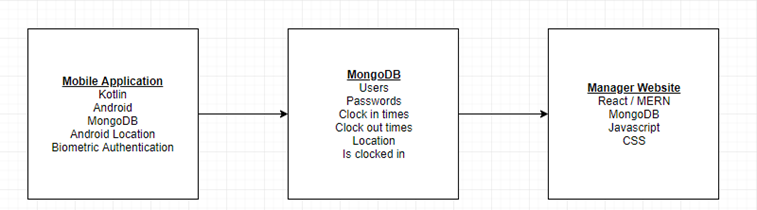
\includegraphics[width=1\textwidth]{img/design.png}
    \caption{Application Design.}
    \label{fig}
\end{figure}
The above image is a simplified image of our project design overall. We have a mobile application developed using android studio which is coded in Kotlin. This application uses both location and biometric authentication features and stores employee information and accounts on our database in mongo DB. Our database stores information we push up from the application to the database. Here you can clearly see our database is storing our Users, Passwords, Clock-in times and Clock-out times, along with the workplace location and if the employee is currently clocked-in.
Our manager website is used by people in management positions inside of the company using the clock in application. Our website is hosted on Heroku and uses WWwhisper to add security to the site. Approved users are emailed, and token given access through their email. This stops people who are not authorized seeing employee information and when people clocked in and out. This is a great security feature and offers employees great peace of mind that their information is stored securely within our database and website.
\\
\section{Application Architecture}
In our final year project, building our app from scratch was not as straight forward as it looked. There was a lot of work put into designing the architecture of the final year project and the application as a whole so that we had it properly planned on how we were going to get all of the components and different features to work as one whole working application. 
\\
\\
The purpose of this app is that the employee is able to clock in and out their times that they have arrived to the workplace instead of signing a sign in form and the manager is able to see which employee clocked in or out by their username and what exact time they actually came into the workplace and what time they finished at in order for the manager to see if the employees are turning up for work on time or not.
\\
\\
So if the employee is after arriving in the workplace, they must immediately clock in on the app so they’re signed in for work. Then the location feature must check if the employee is in the workplace and if they are found to be there, then they are brought into the log in feature. They must be already signed up to this feature and if not they must set up an account containing their email, password and their fingerprint. If the user does have an account then they have to log in using their name and password. After that then a fingerprint recognition system comes in and they have to use their fingerprint in order to complete the clock in. If the employee’s fingerprint is the right match then they are brought into the clock in feature. Then they are able to press the clock in button which automatically clocks the employee into work and the details of their clock in is immediately stored in the database.
\\
\\
The employee will then be able to clock in their breaks from work and will clock in again when they have returned to work from their break. The clock out feature then will be used for when the employee feature is finished at work for the day. The employee will have to clock out and will most likely sign out from the app as well.
\\
\\
The clock in, clock out and break times then are able to be viewed by the manager through the database that’s connected to the application. The manager has it’s own feature where they are able to log in on the website where they have the access to the database where they are able to see all the details of the employee’s. The manager is able to see who the employee is and at what time they either clocked in or out and how long they took their break from work. This is great way for the manager to see if his employees are turning up for work and if they are fulfilling their work duties which are required for them to do.

\subsection{Login Page}
\begin{figure}[h]
    \centering
    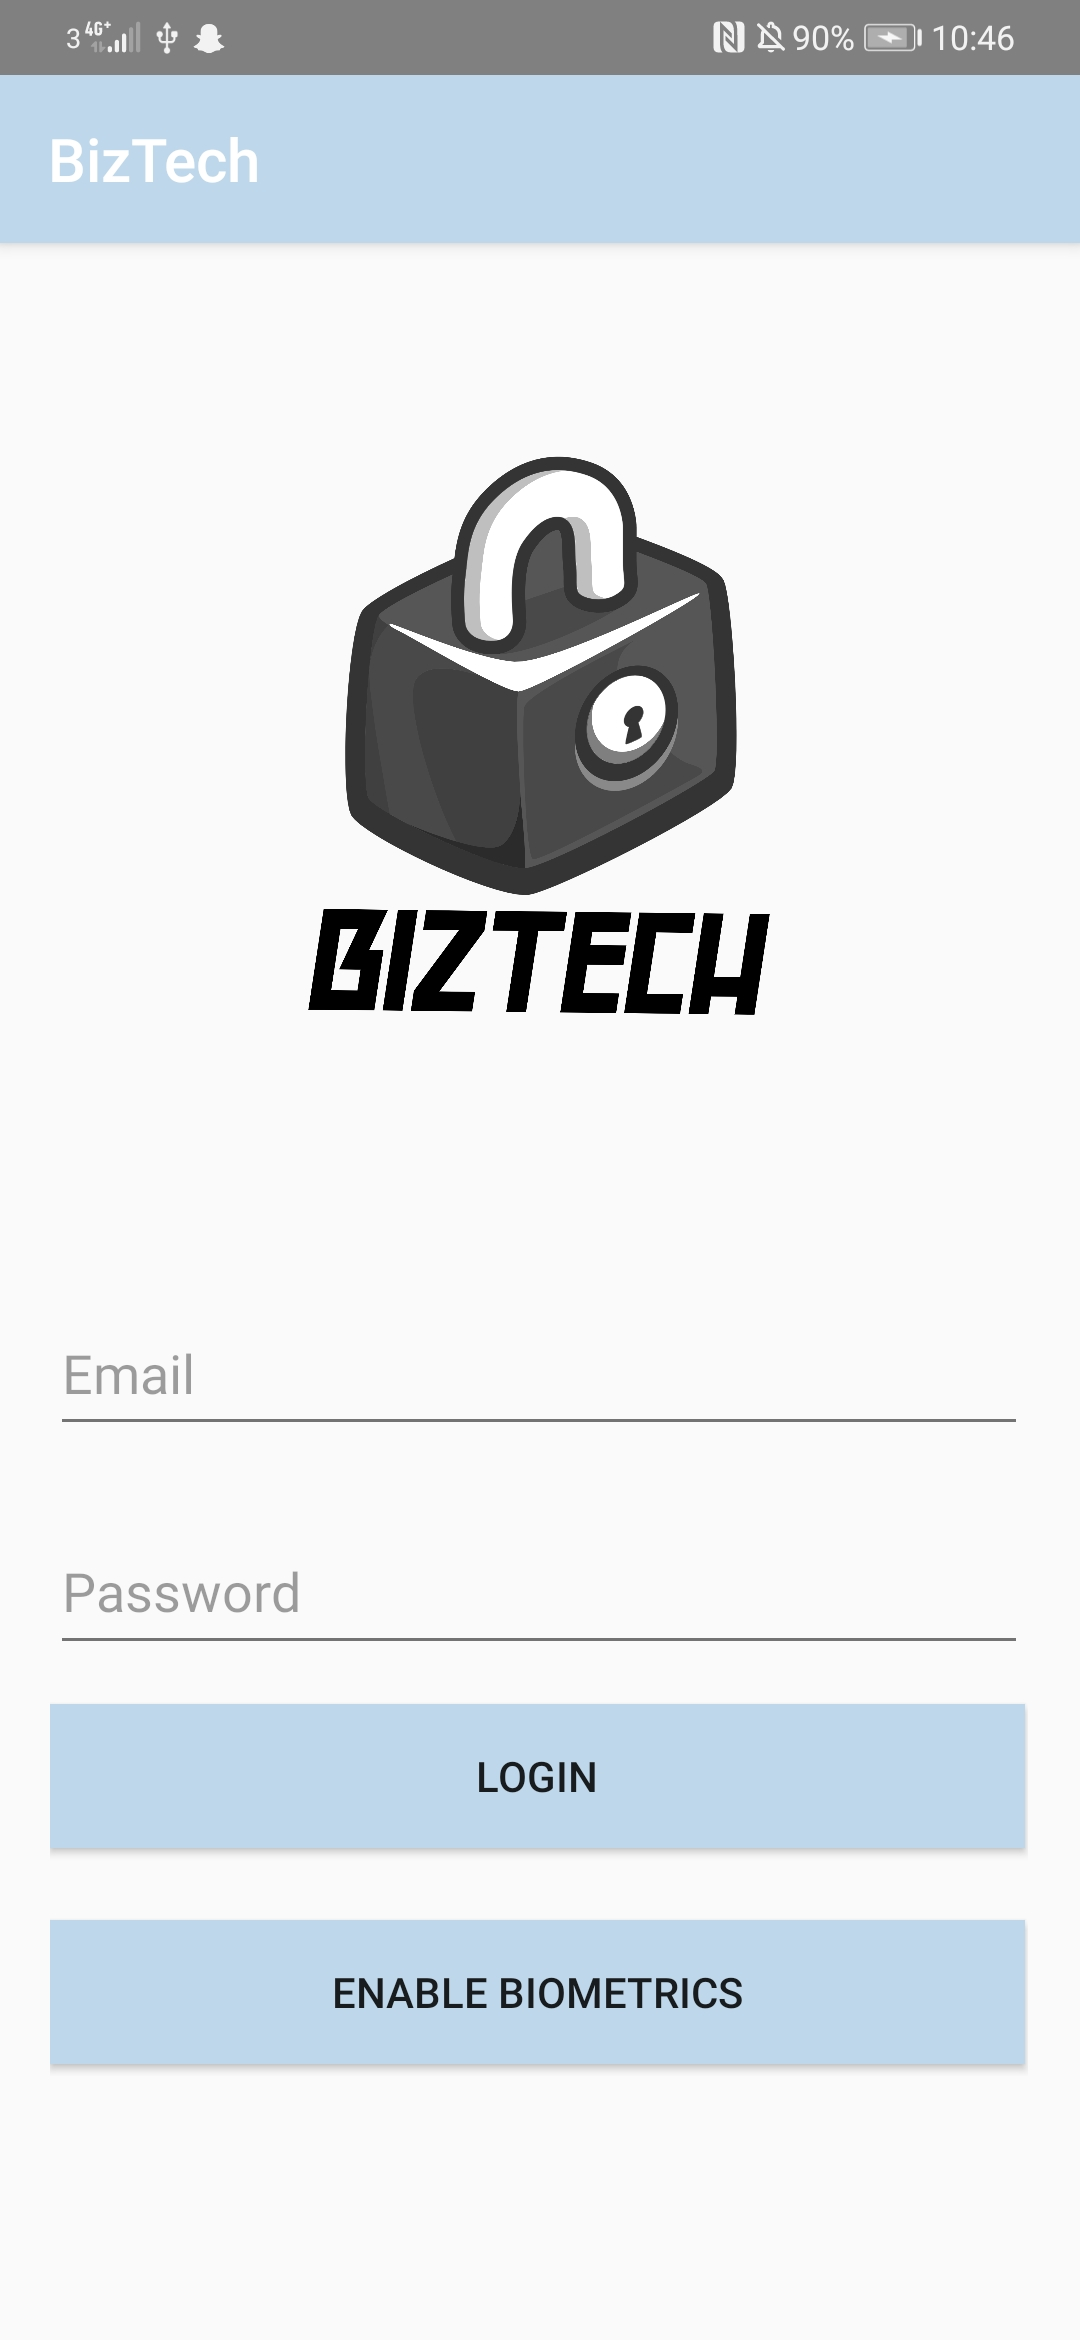
\includegraphics[width=0.5\textwidth]{img/LoginPage.jpg}
    \caption{Login Page.}
    \label{fig}
\end{figure}
The image shown in \textbf{figure 5.2} shows our applications login page. This is the page seen by both managers and employees when the application is first access. Obviously if the person has not had an account made or has had their account removed etc meaning it is no longer on the database they will not be able to login. Once logged in the user will have access to the clock in application. As stated before in this document if the user is not within the specified location which is set by management they will not be able to clock in meaning they will be restricted to being able to change their password and log out.
\FloatBarrier

\subsection{Home Page}
\begin{figure}[!htb]
    \centering
    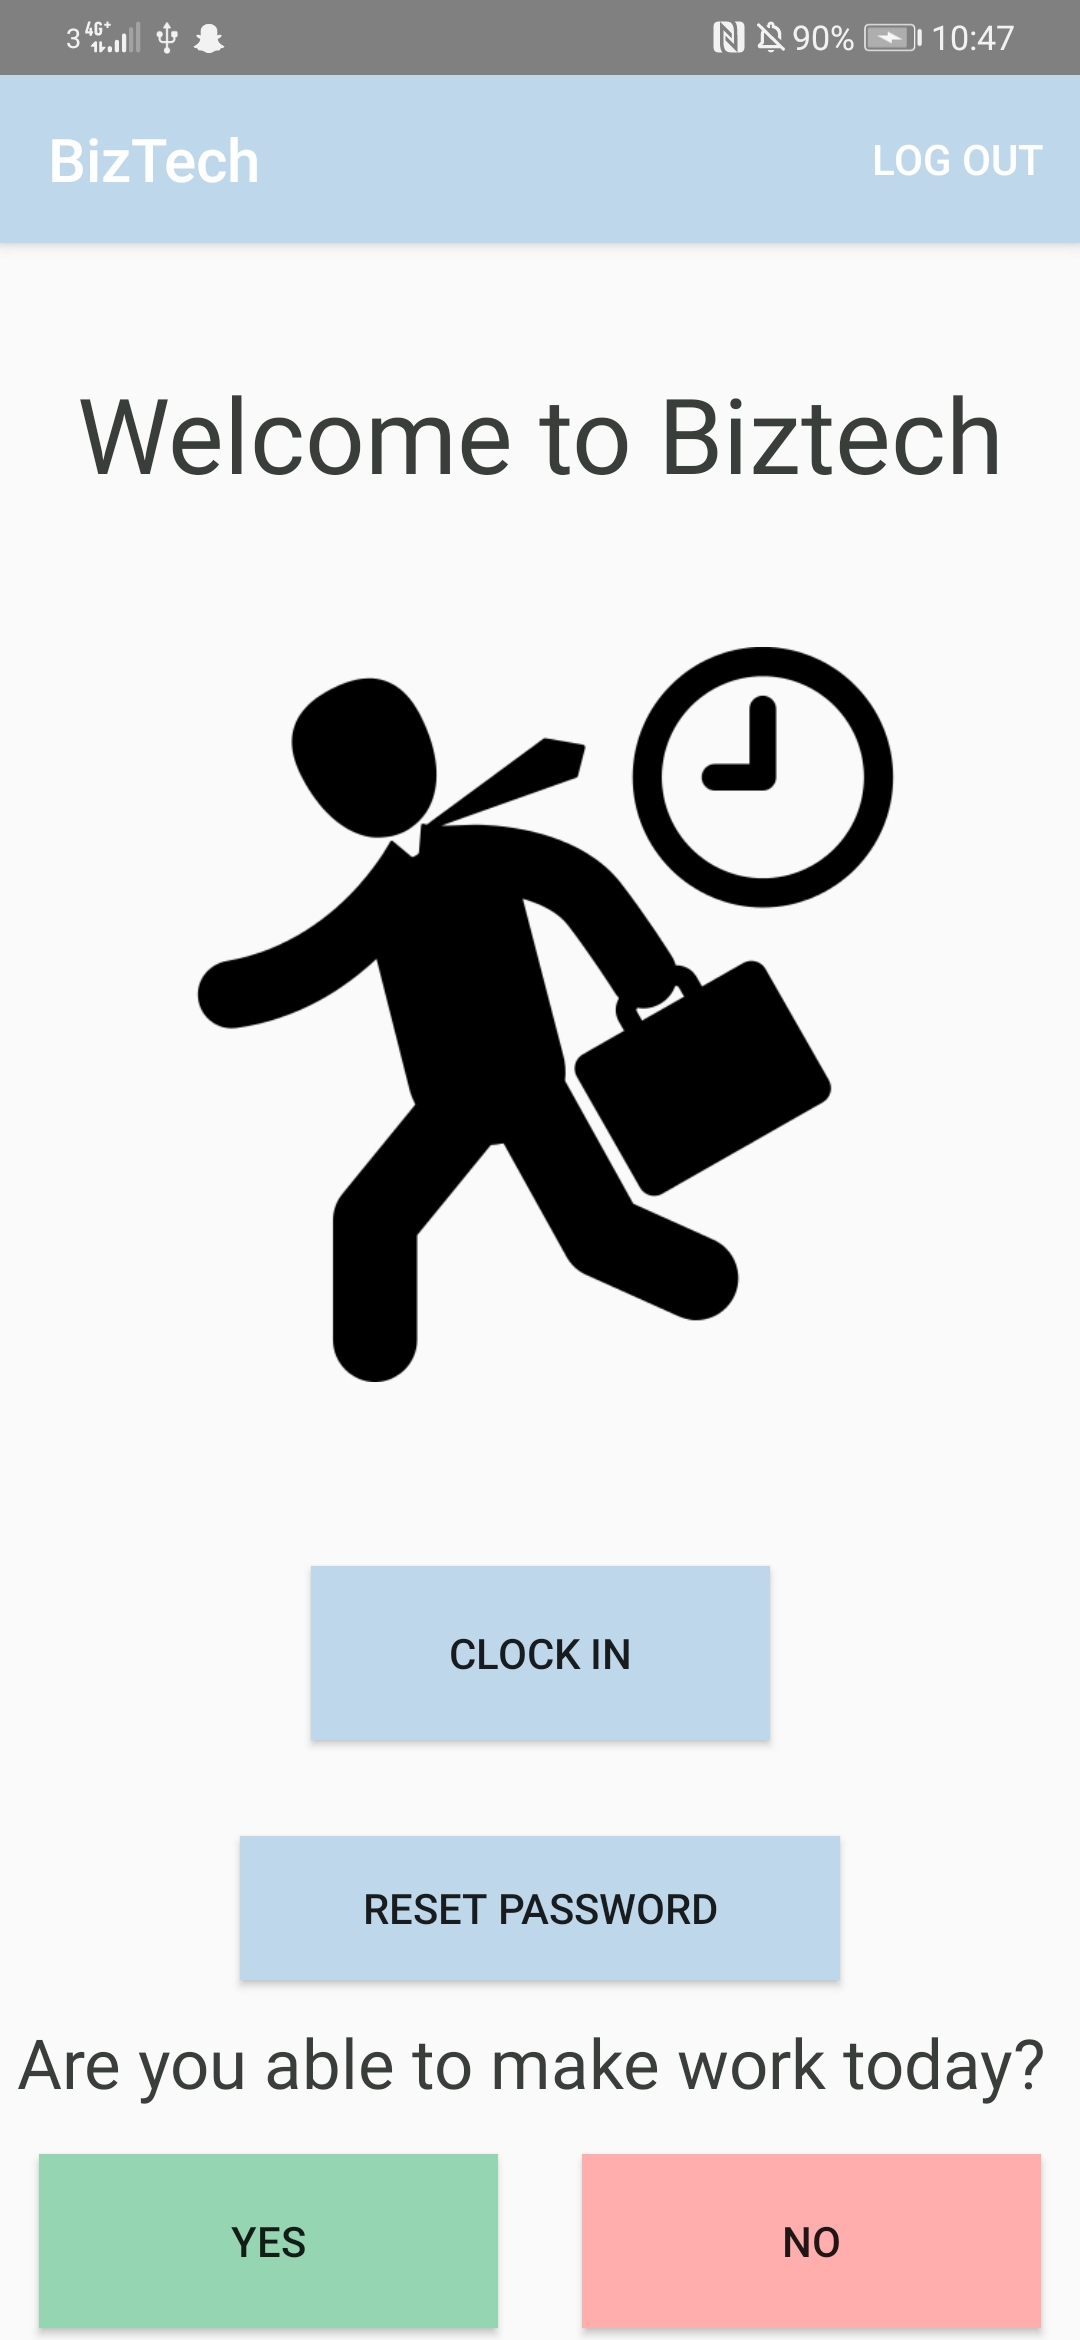
\includegraphics[scale=0.15]{img/ClockInPage.jpg}
    \caption{Clock In Page.}
    \label{fig}
\end{figure}
The image shown in \textbf{Figure 5.3} shows the page that the user will see when he first logs in to the application. There is a Log Out button in the top left of the screen which when pressed will Log the employee out of the application. The clock in button will be disabled for 6 seconds and this is due to the application connecting to the MongoDB database. There is also a reset password button which when pressed the employee can reset their password. The last feature we have decided to include was the sickness button so if an employee is unable to attend work if the employee clicks the No button then this will be displayed on the website so the manager will know employees who are sick and not able to attend work. This is also the clock out page as when the employee clocks out from work they will be brought back to this page.
\FloatBarrier

\subsection{Clocked In / Clocked Out Page}
\begin{figure}[!htb]
    \centering
    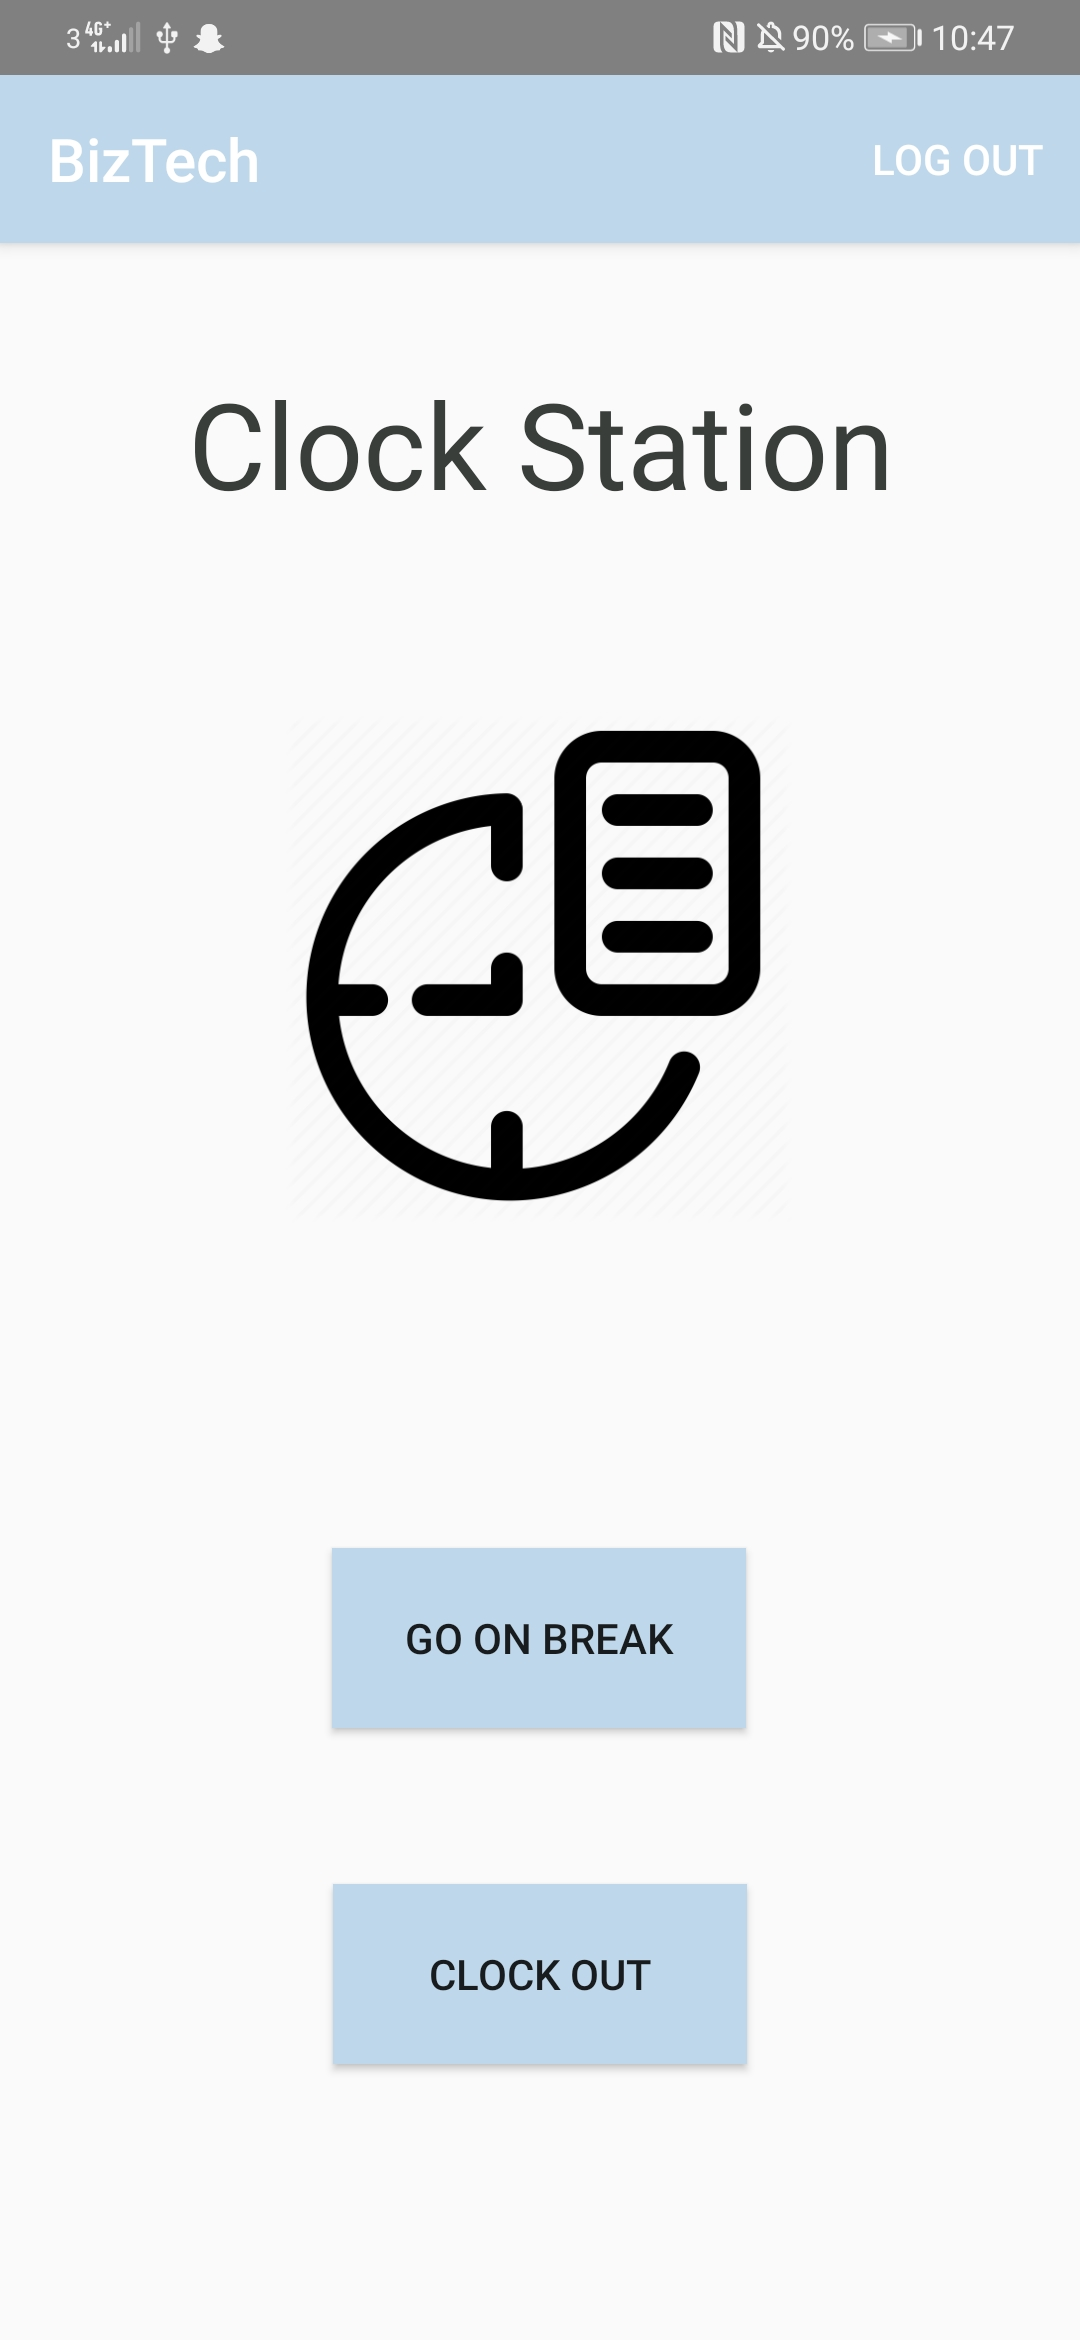
\includegraphics[scale=0.15]{img/ClockedInPage2.jpg}
    \caption{Clock In Page.}
    \label{fig}
\end{figure}
The image shown in \textbf{Figure 5.4} shows the Clocked In / Clocked out page so when the employee presses the Clock in button on the home page they will be navigated to this page so the employee is now clocked into work and they have two options on this page which are go on break or to clock out of work. If the employee was to press the go on break button it would bring them to the break page or they can clock out and then they will be navigated back to the clock out page.
\FloatBarrier

\subsection{Break Page}
\begin{figure}[!htb]
    \centering
    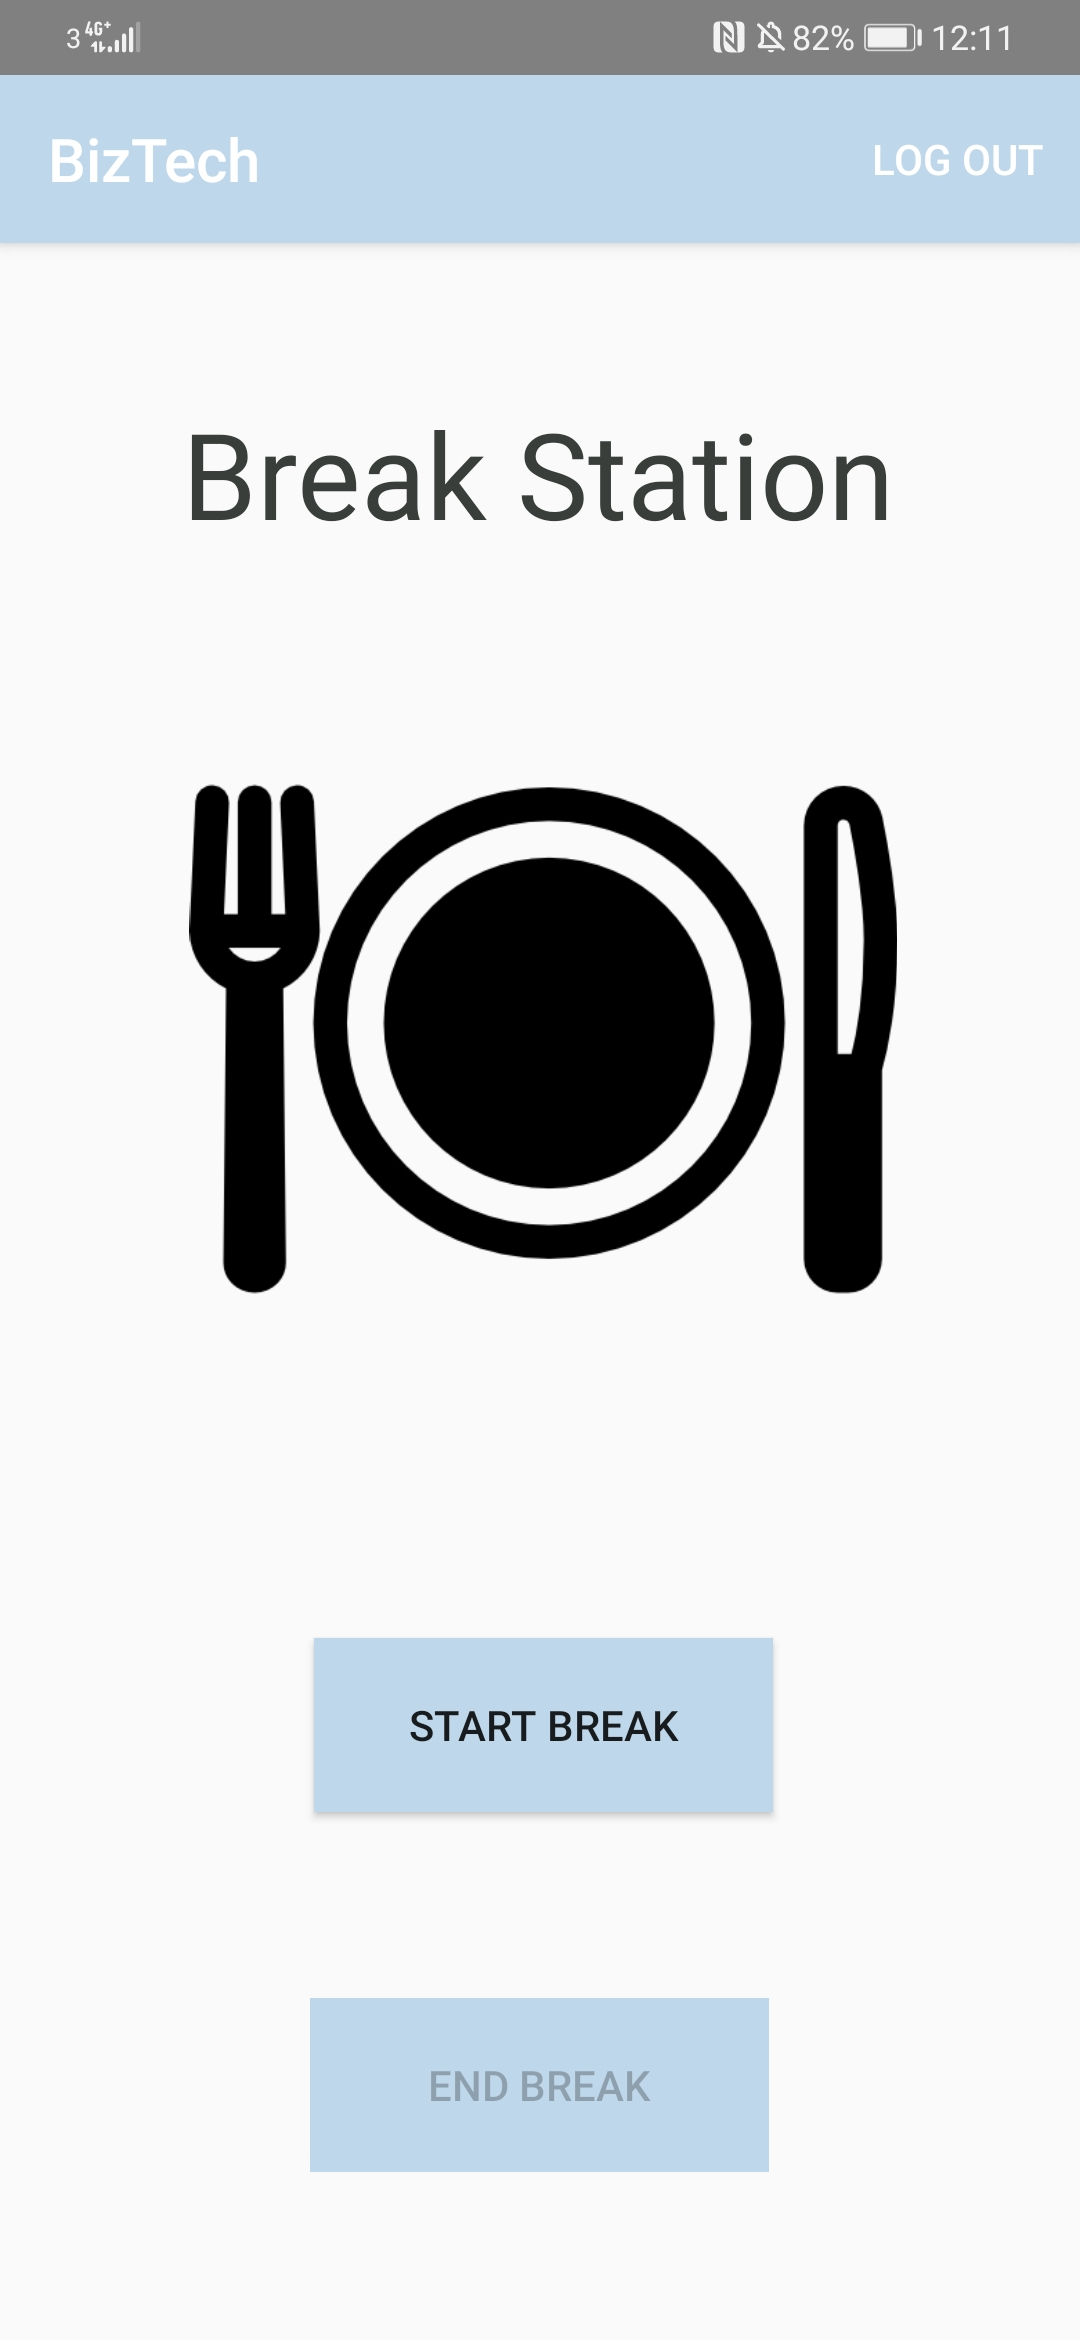
\includegraphics[scale=0.15]{img/BreakPage.jpg}
    \caption{Break Page}
    \label{fig}
\end{figure}
The image shown in \textbf{Figure 5.5} is the page you will be prompted to when the go on break button is pressed after the clock in button is pressed. This is a simple page that lets the employee start there break and the employee can't end their break without starting their break. When the start break button is pressed this is sent straight to the database and then displayed on the website and then when the end break button is pressed the same process happens. After pressing the end break button then you will be brought back to the clocked in page.
\FloatBarrier

\subsection{Manager Area}
\begin{figure}[!htb]
    \centering
    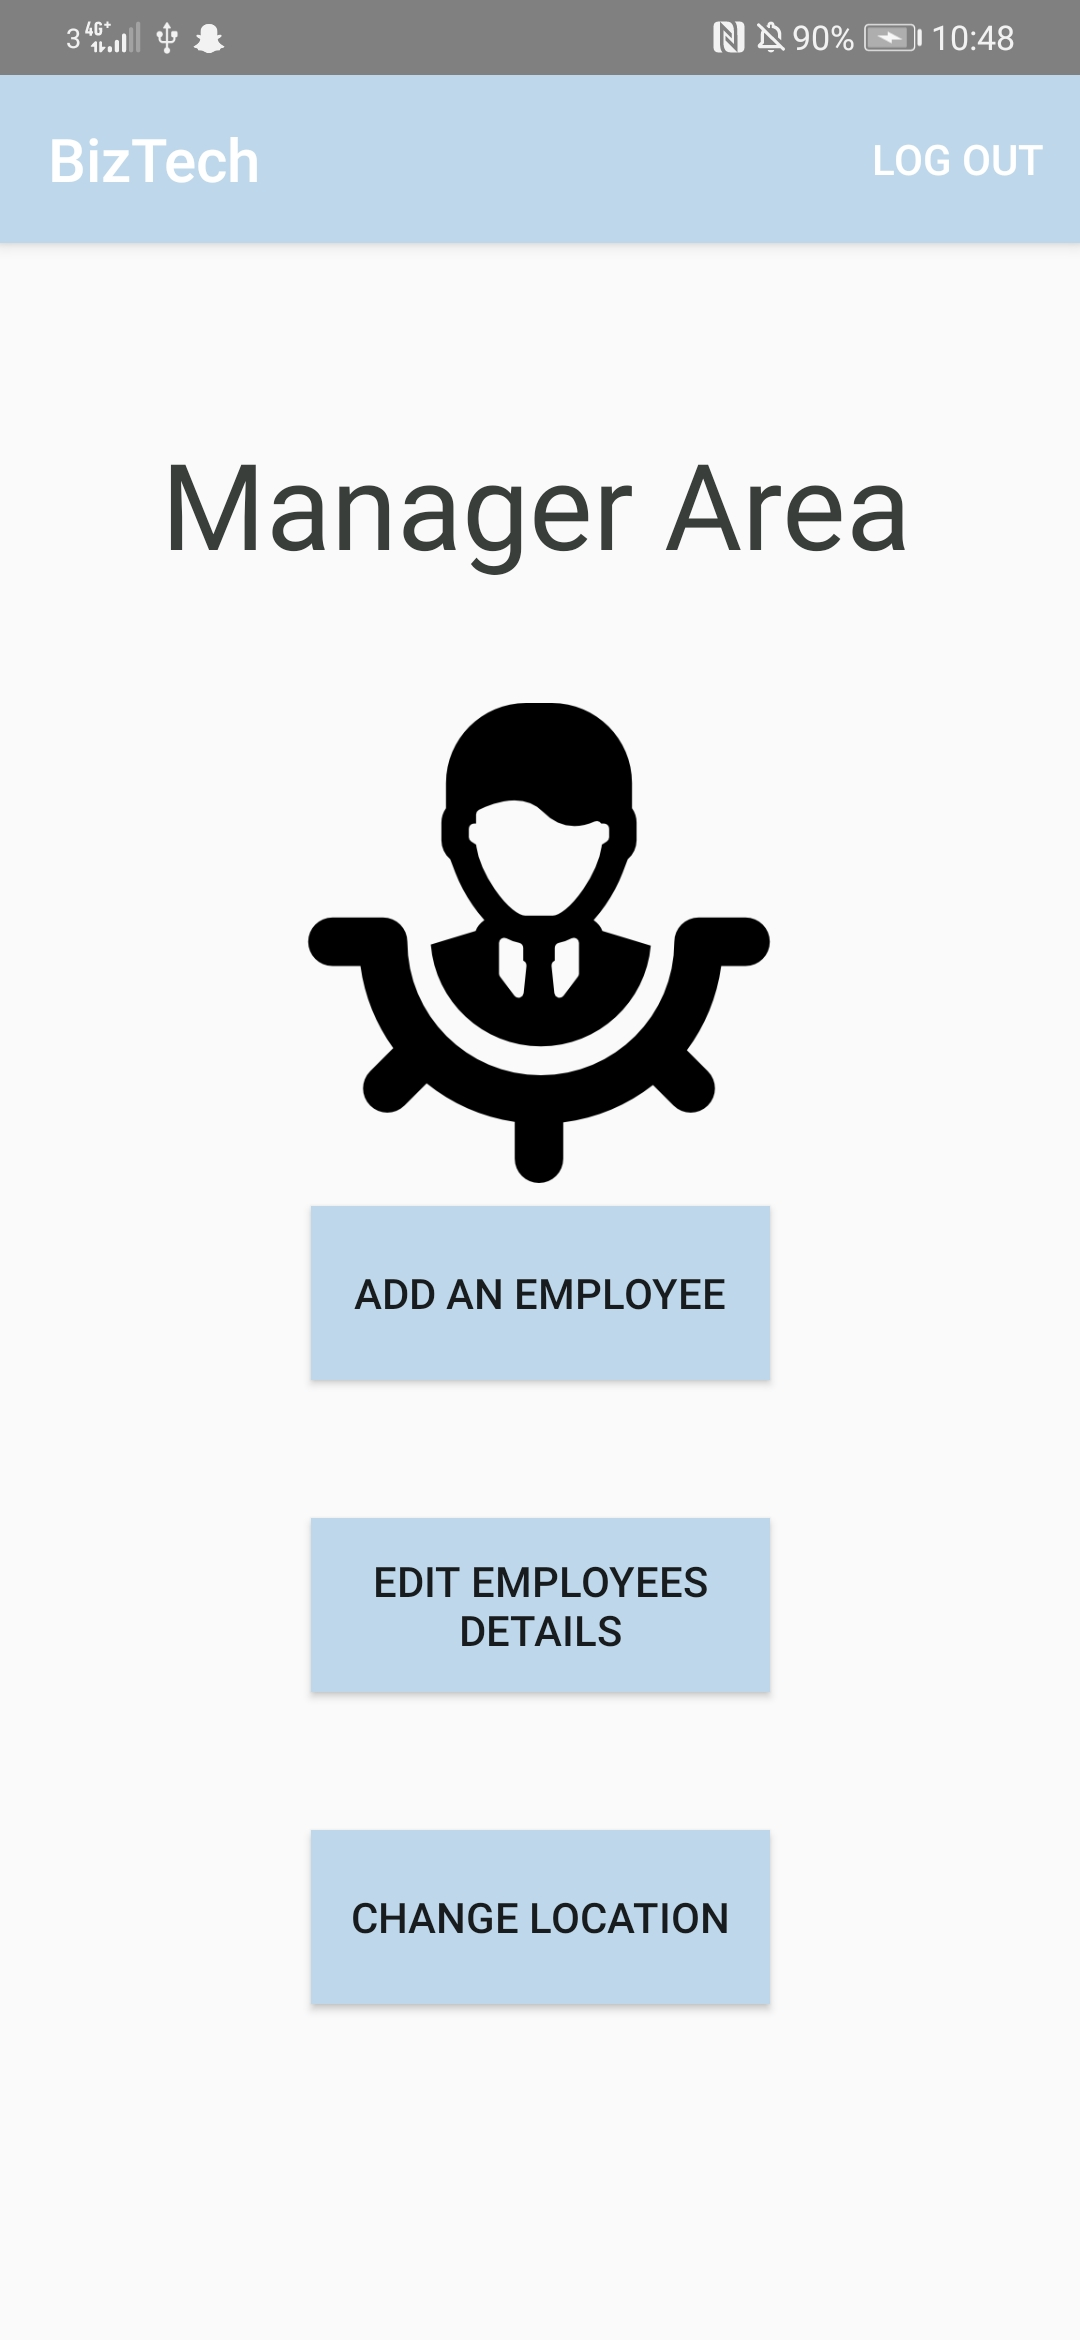
\includegraphics[scale=0.15]{img/ManagerAreaPage.jpg}
    \caption{Manager Area Page}
    \label{fig}
\end{figure}
In \textbf{figure 5.6} we see the admin homepage area. Once you have logged in as an admin this is what screen you are met with. Firstly, you can see the log out button in the top right. Clicking this button will log you out of the application and bring you back to the login in screen. As you can see on this page there is three buttons which all bring you to different areas where different settings and information can be changed. This area and all these settings is only accessible by managers who log in.
\FloatBarrier


\subsection{Create Employees}

\begin{figure}[!htb]
    \centering
    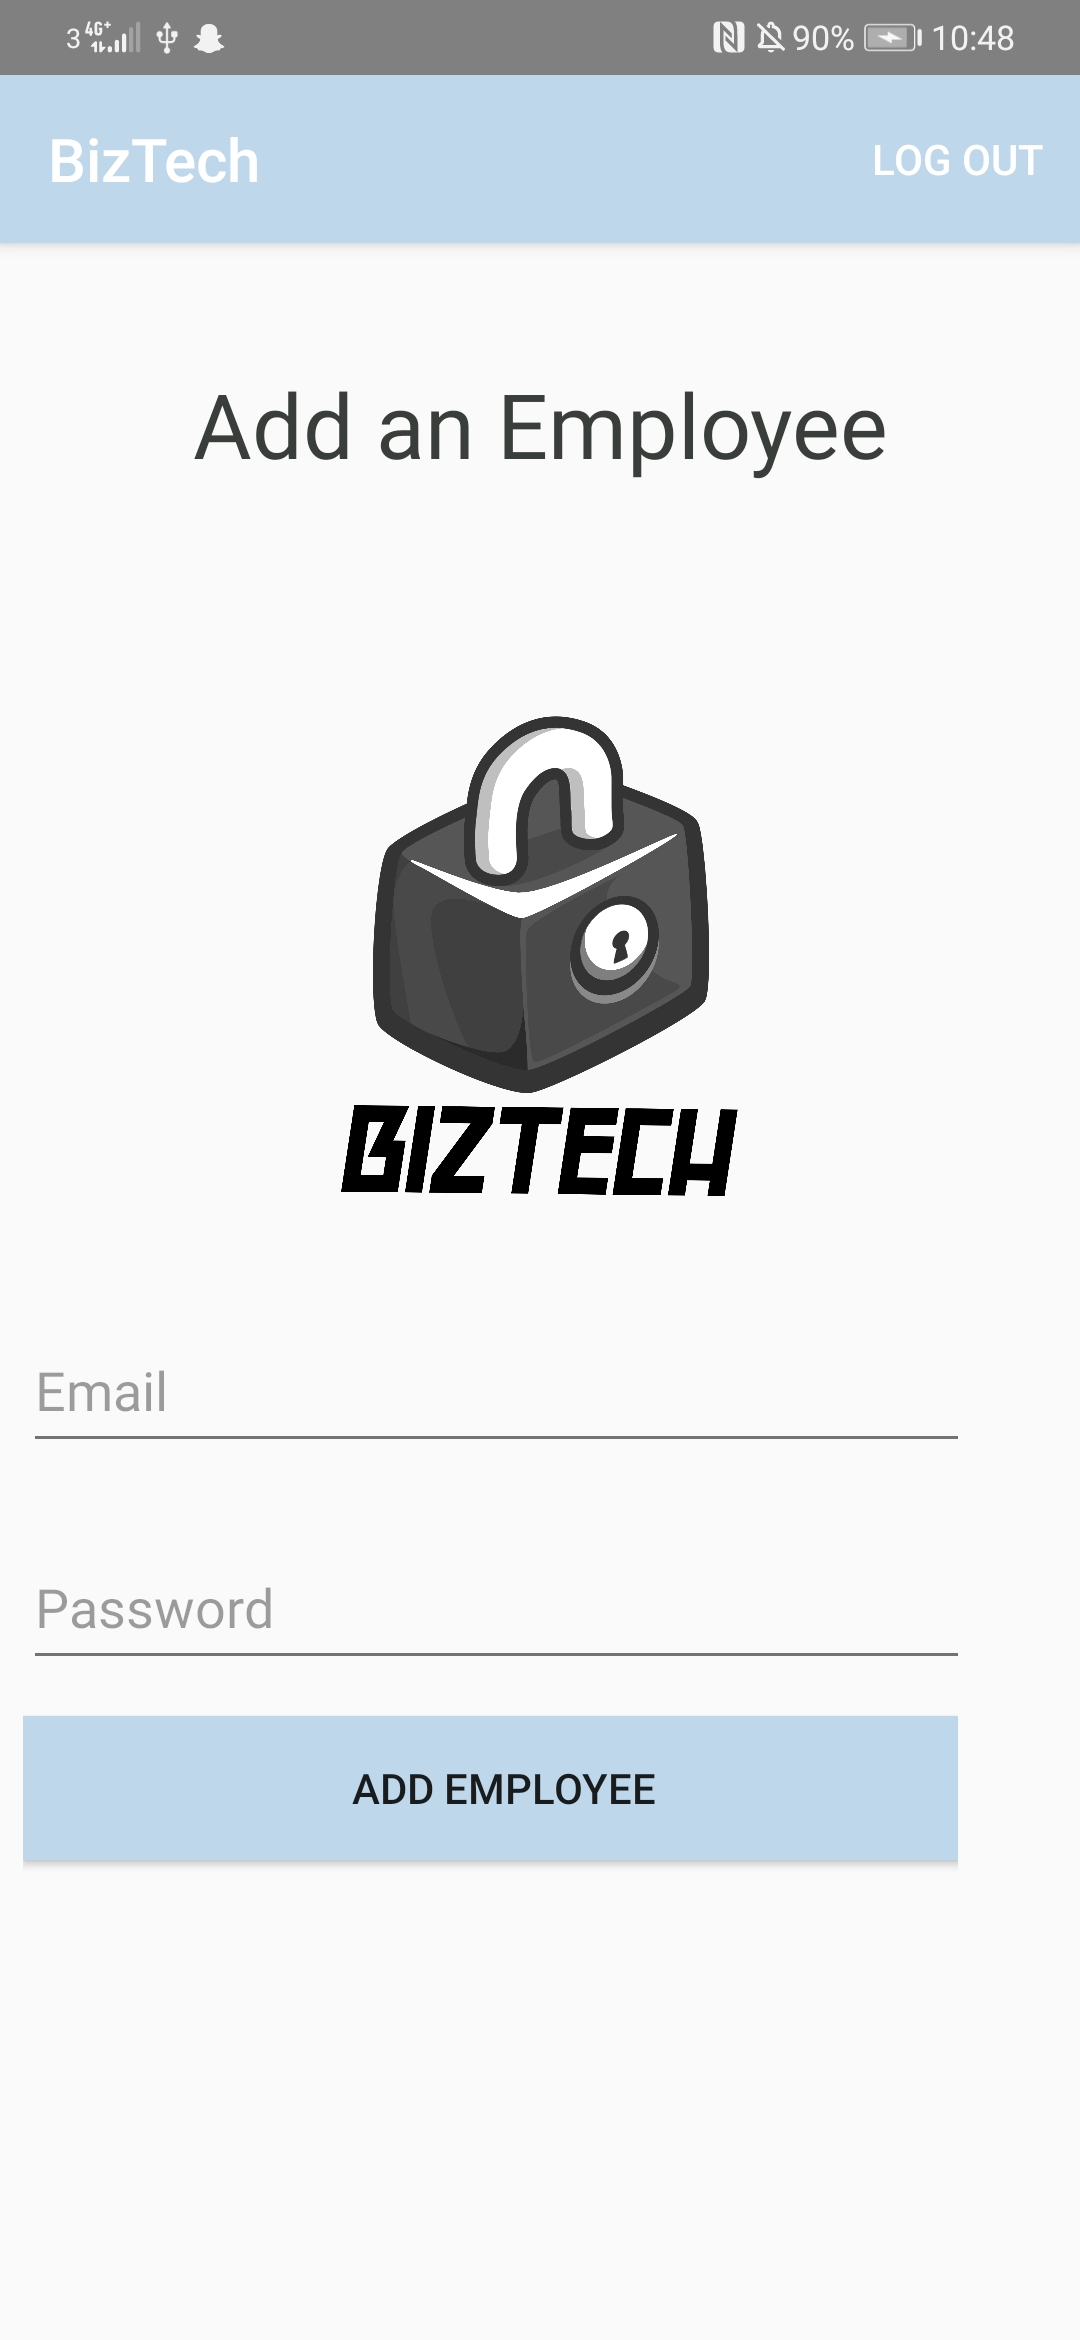
\includegraphics[scale=0.15]{img/AddNewEmployeePage.jpg}
    \caption{Create Employee}
    \label{fig}
\end{figure}

\textbf{Figure 5.7} shows the create employee page. This page is where managers can create an employee’s account in order to allow them to use the application. We designed this in such a way that employees accounts would be made by the manager and once made the employee can change the password set for them when their account was made. Managers in workplaces are the people whom carry out the interviews and accept new employees in most cases so we as a team felt it the right decision to leave creating the accounts up to the managers as we didn’t want people who didn’t work in the workplace to be able to create accounts as this could lead to empty used accounts and a huge amount of accounts when there isn’t as many employees. on the MongoDB.
\FloatBarrier

\subsection{Edit employee details}
\begin{figure}[!htb]
    \centering
    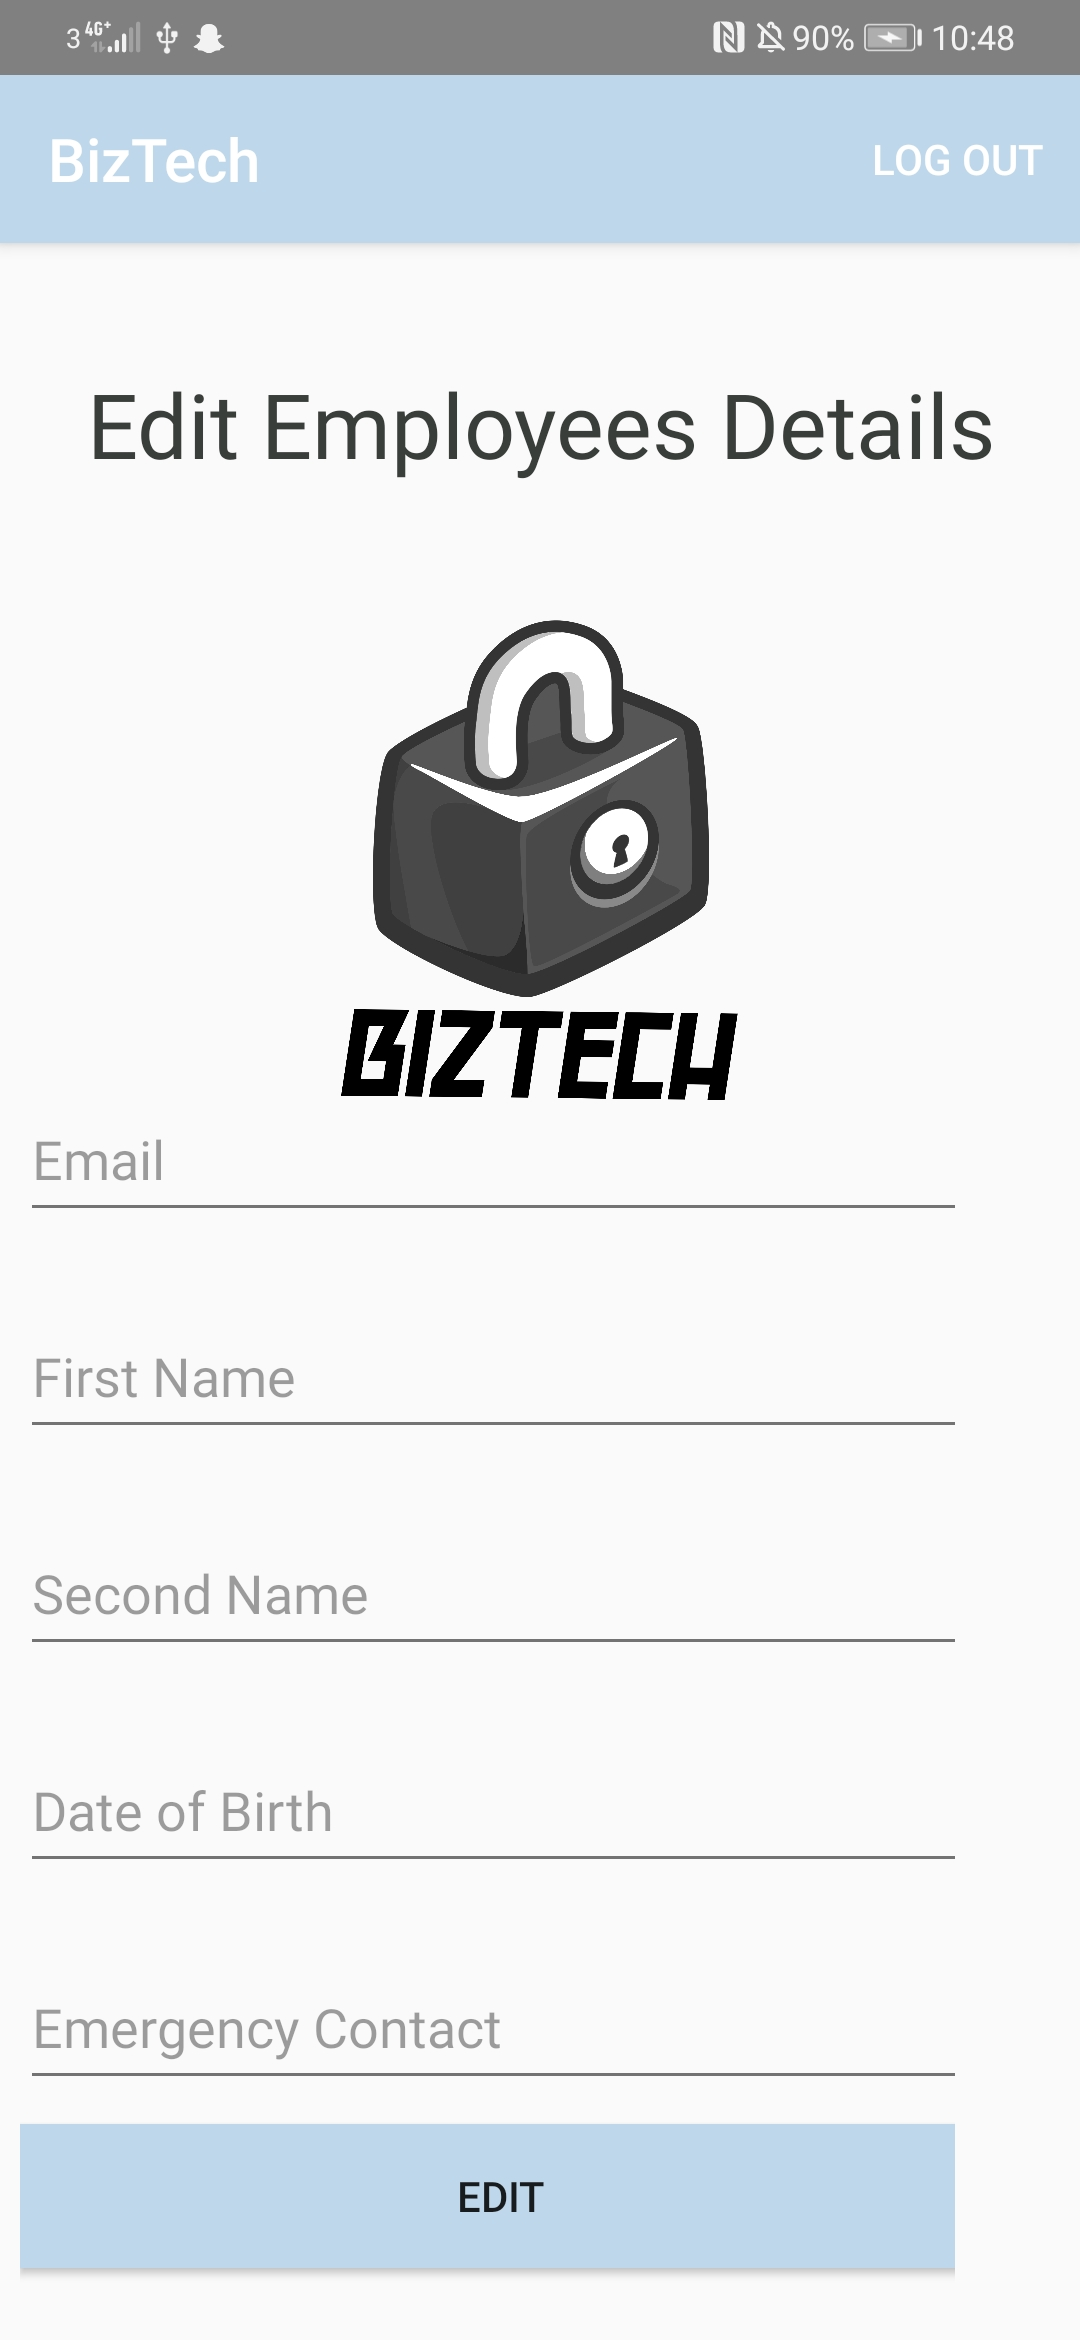
\includegraphics[scale=0.15]{img/EditEmployeeDetailsPage.jpg}
    \caption{Edit Employee Details}
    \label{fig}
\end{figure}

\textbf{Figure 5.8} shows employee details page. On this page managers can make changes to the employee’s details whether it be changing their name, date of birth email or emergency contacts. This is very useful as it allows the manager to change details stored on the database whether it is due to and error when they are inputted or if a number or email has changed. Emergency contact was a thing we as a team agreed fully on and we believe this is a great idea as if anything was to happen in the workplace managers will be able to see emergency contacts of the employees in a matter of seconds.
\FloatBarrier

\subsection{Change Location}
\begin{figure}[!htb]
    \centering
    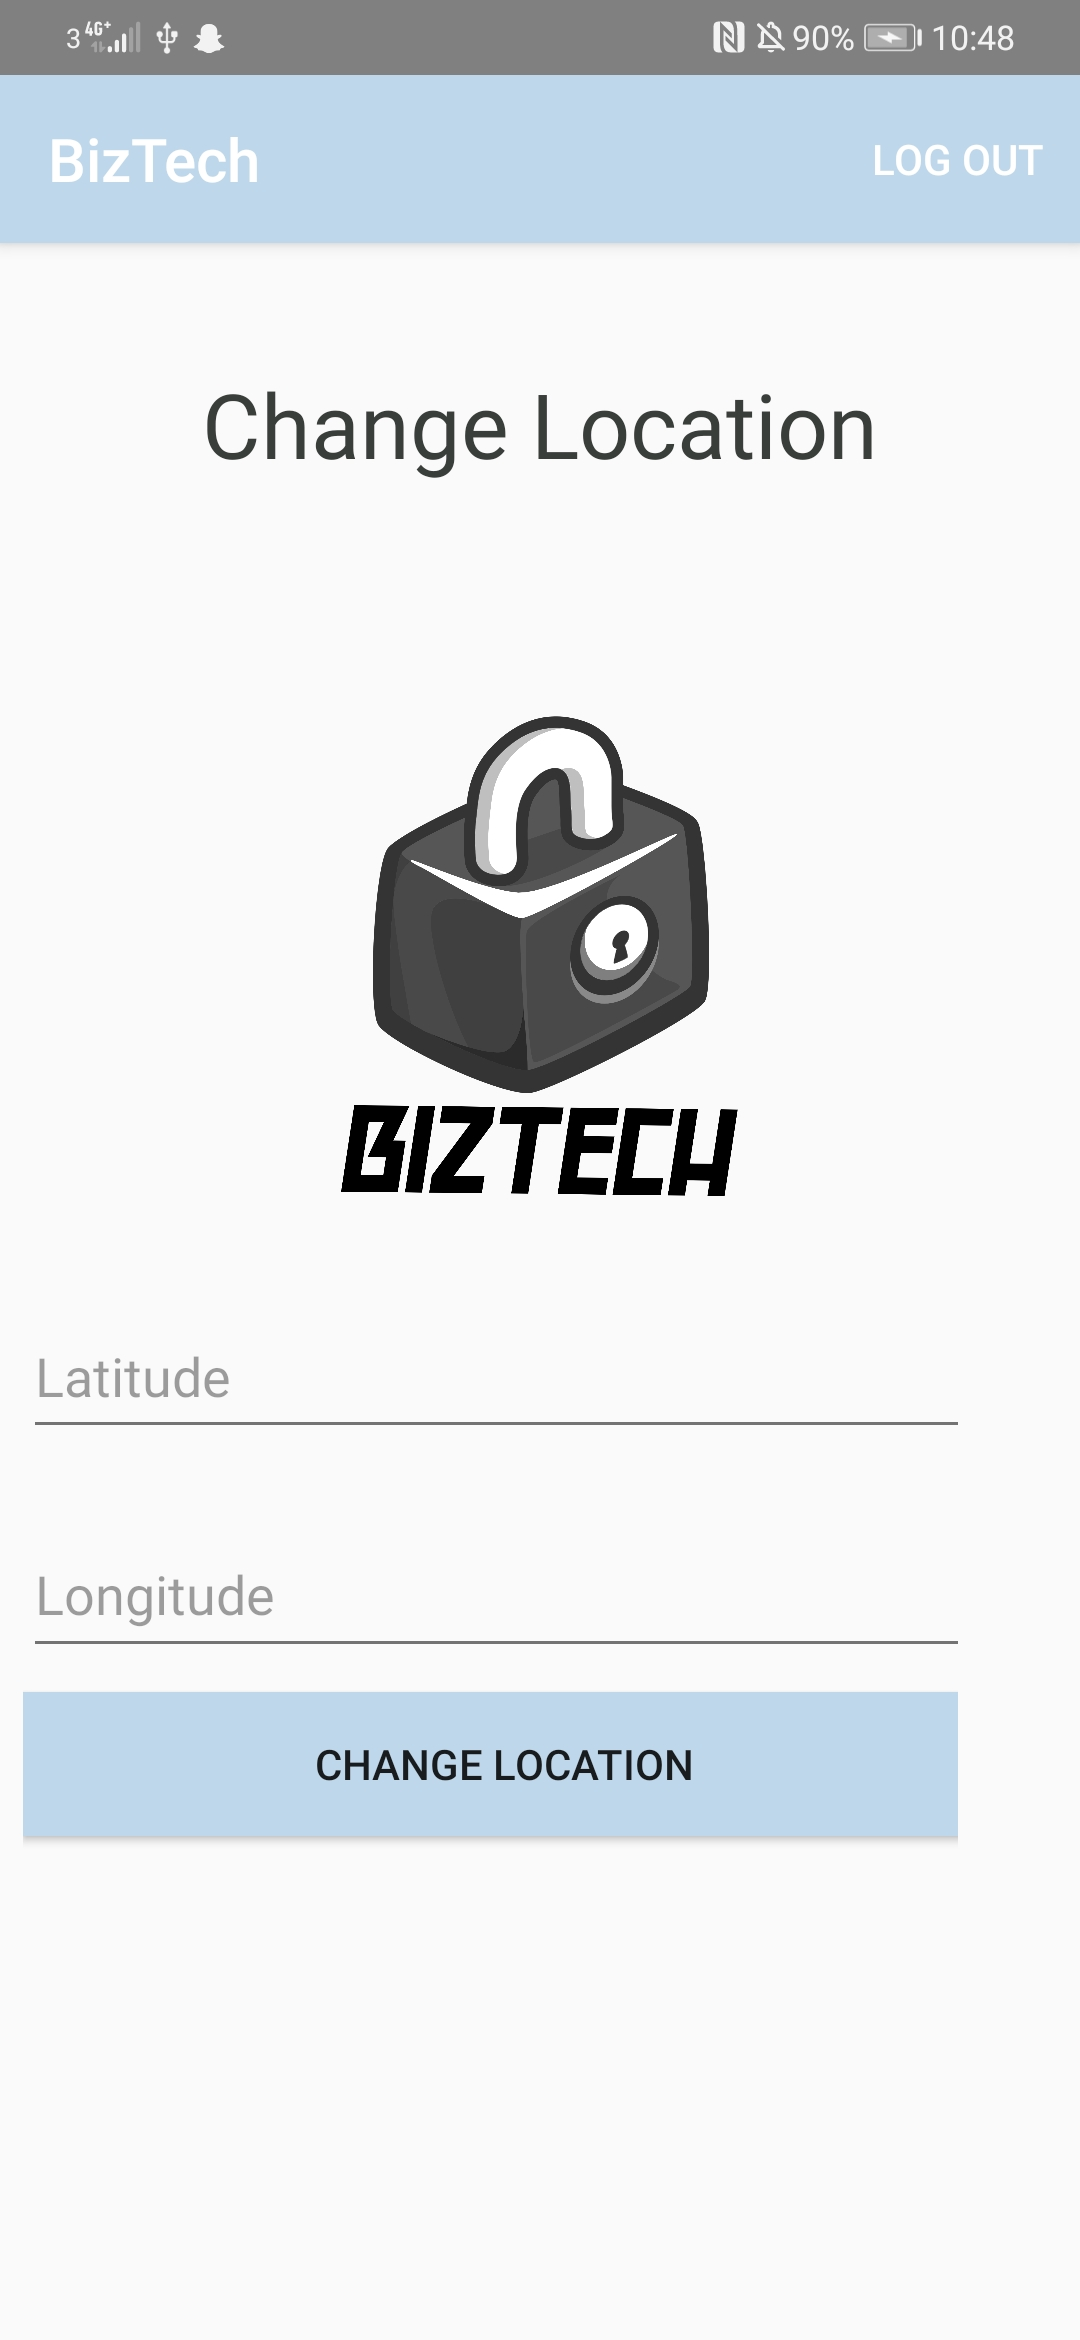
\includegraphics[scale=0.15]{img/ChangeLocationPage.jpg}
    \caption{Change Location}
    \label{fig}
\end{figure}
In \textbf{figure 5.9} we can see what the change location page looks like. Again, it has the log out button located in the top right of the screen which will log the user out and bring them back to the homepage where they can log back in. In the input boxes we can see the placeholder text clearly. The top box is for your latitude and the bottom box is for the longitude. Changing this will change the workplace area and will impact how and when people can clock into the workplace. Changing the location should not have to be done very often. Changing this location will also change the location of the workplace stored on the MongoDB.
\FloatBarrier

\section{Website Architecture}

\subsection{Clock In Times}
\begin{figure}[!htb]
    \centering
    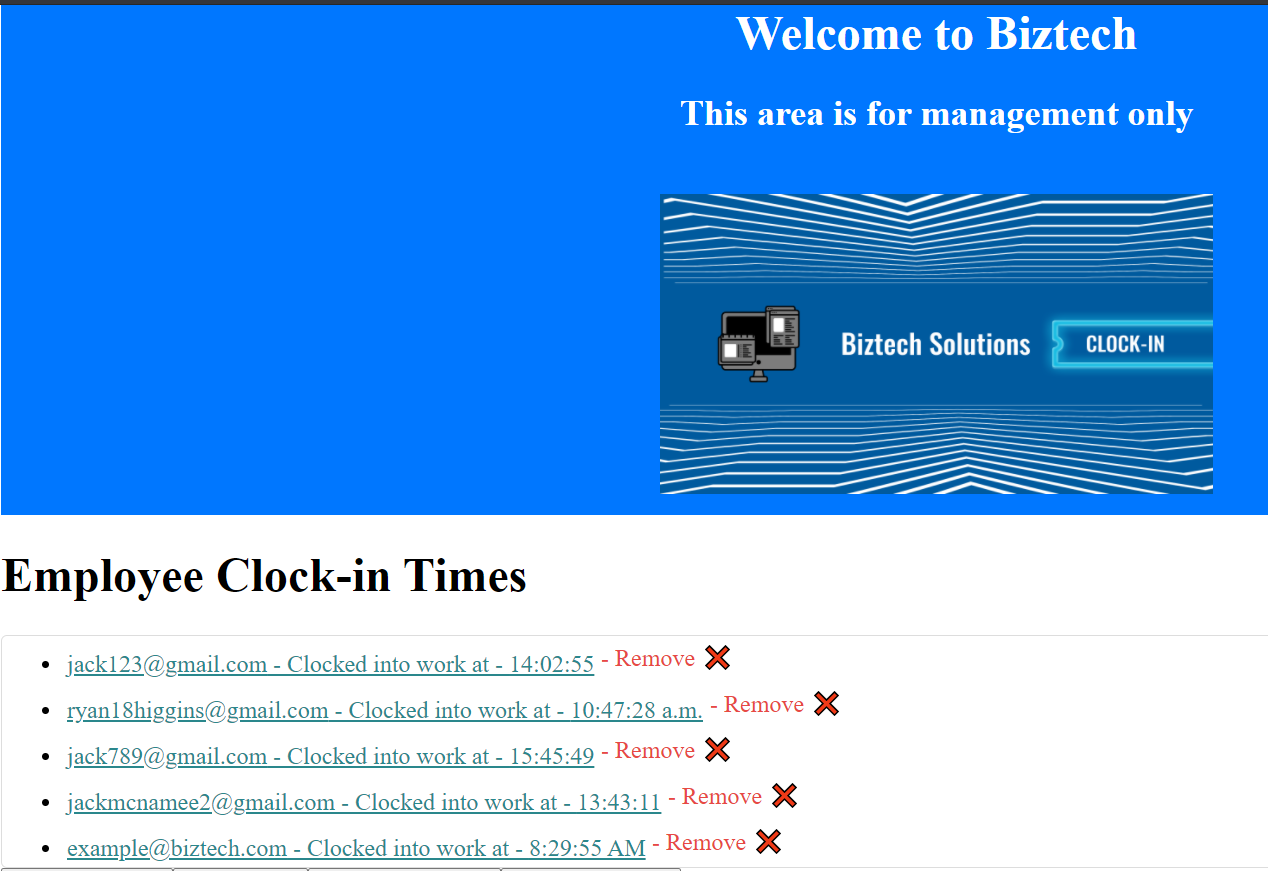
\includegraphics[scale=0.66]{img/ClockInTimes.PNG}
    \caption{Clock In Times}
    \label{fig}
\end{figure}
\textbf{Figure 5.10} shows the clock in times displayed to the manager on the website. This is where a manager can come to see who clocked into work and whether they were late or on time. The records update themselves and do not duplicate so each employee will only have 1 entry rather than 7 per week. This helps to keep the table clean and easy to read.
\FloatBarrier

\subsection{Clock Out Times}
\begin{figure}[!htb]
    \centering
    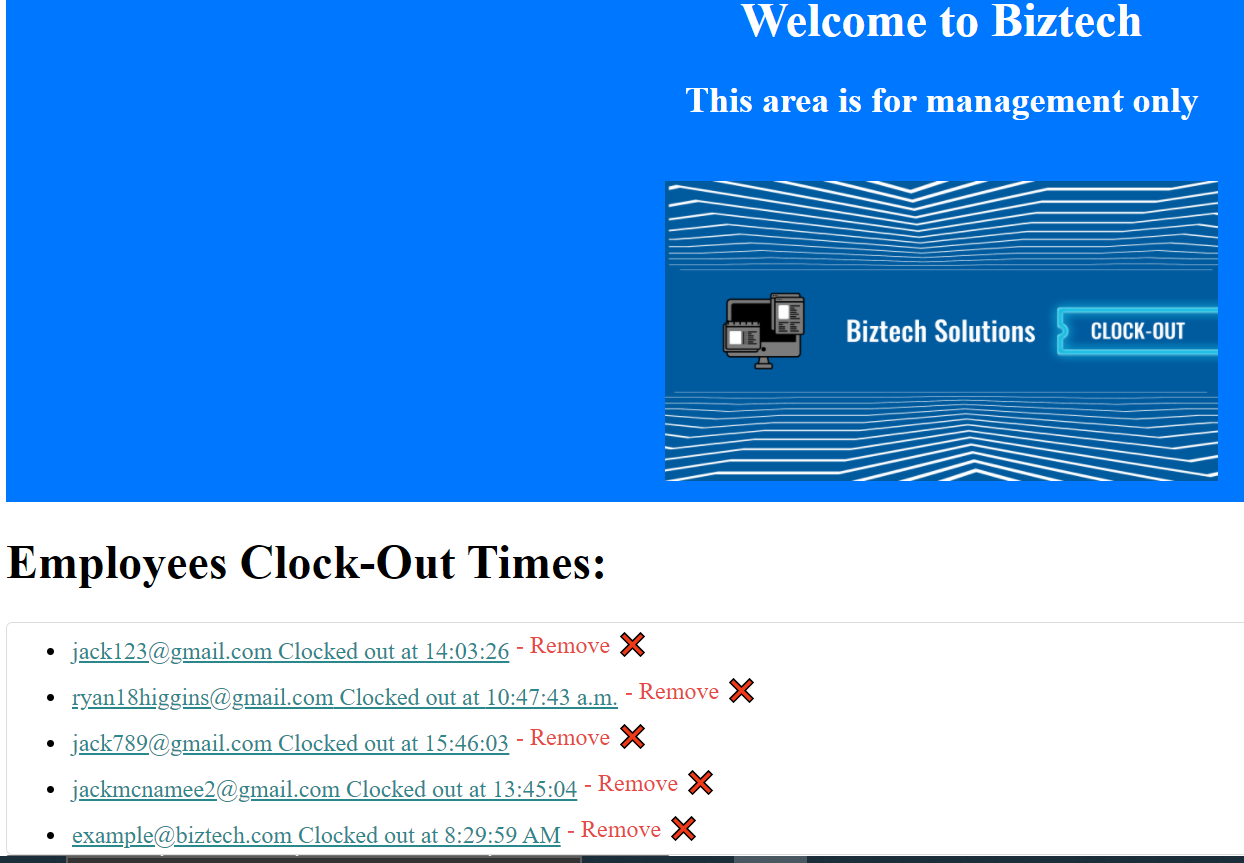
\includegraphics[scale=0.66]{img/ClockOutTimes.PNG}
    \caption{Clock Out Times}
    \label{fig}
\end{figure}
\textbf{Figure 5.11} shows the clock out times displayed to the manager on the website. This is where a manager can come to see who clocked out of work and when. The records update themselves and do not duplicate so each employee will only have 1 entry rather than 7 per week. This helps to keep the table clean and easy to read.
\FloatBarrier


\subsection{Break Times}
\begin{figure}[!htb]
    \centering
    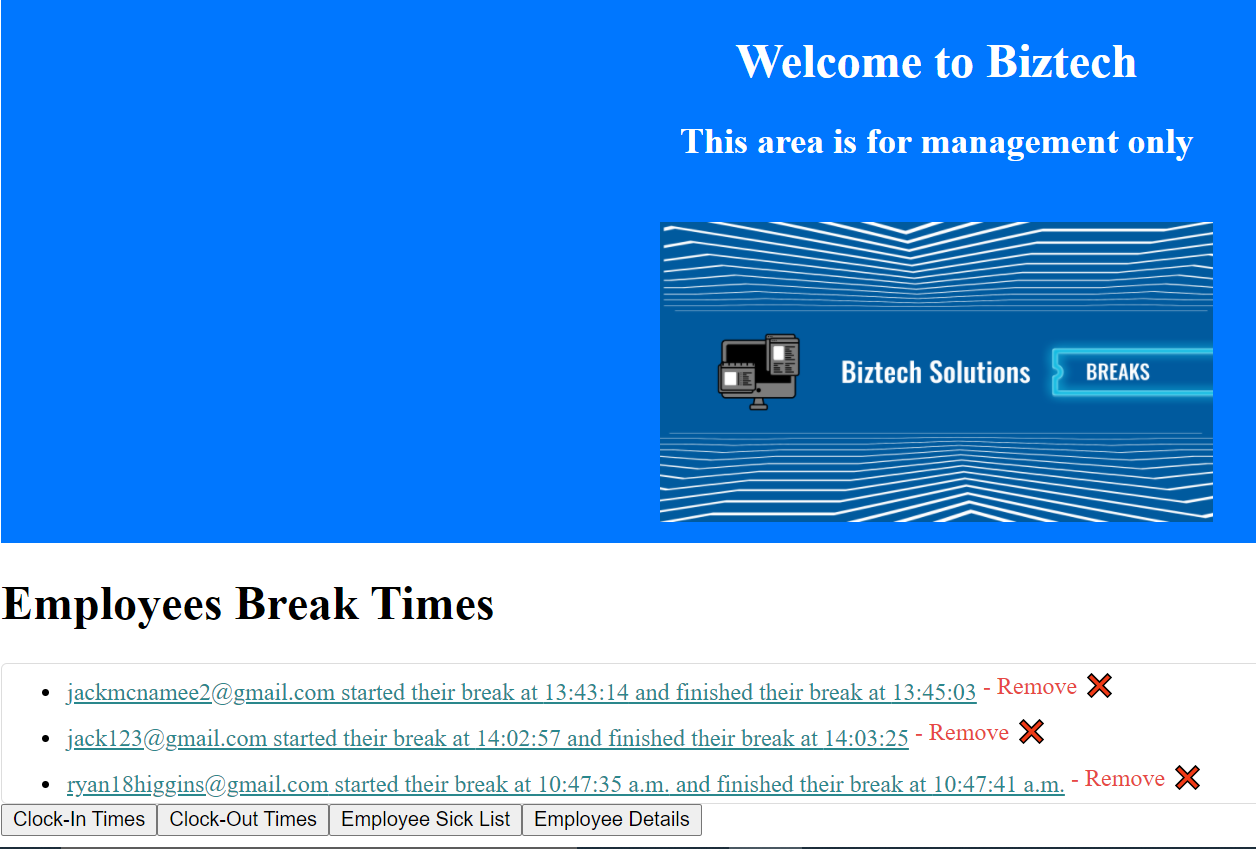
\includegraphics[scale=0.66]{img/BreakTimes.PNG}
    \caption{Clock Out Times}
    \label{fig}
\end{figure}
\textbf{Figure 5.12} displays the employees break times on the website. When the employee starts their break it will say "started their break at " and give the time and if the employee was still to be on break it would display a message on the website saying 
\FloatBarrier

\subsection{Employee details displayed}
\begin{figure}[!htb]
    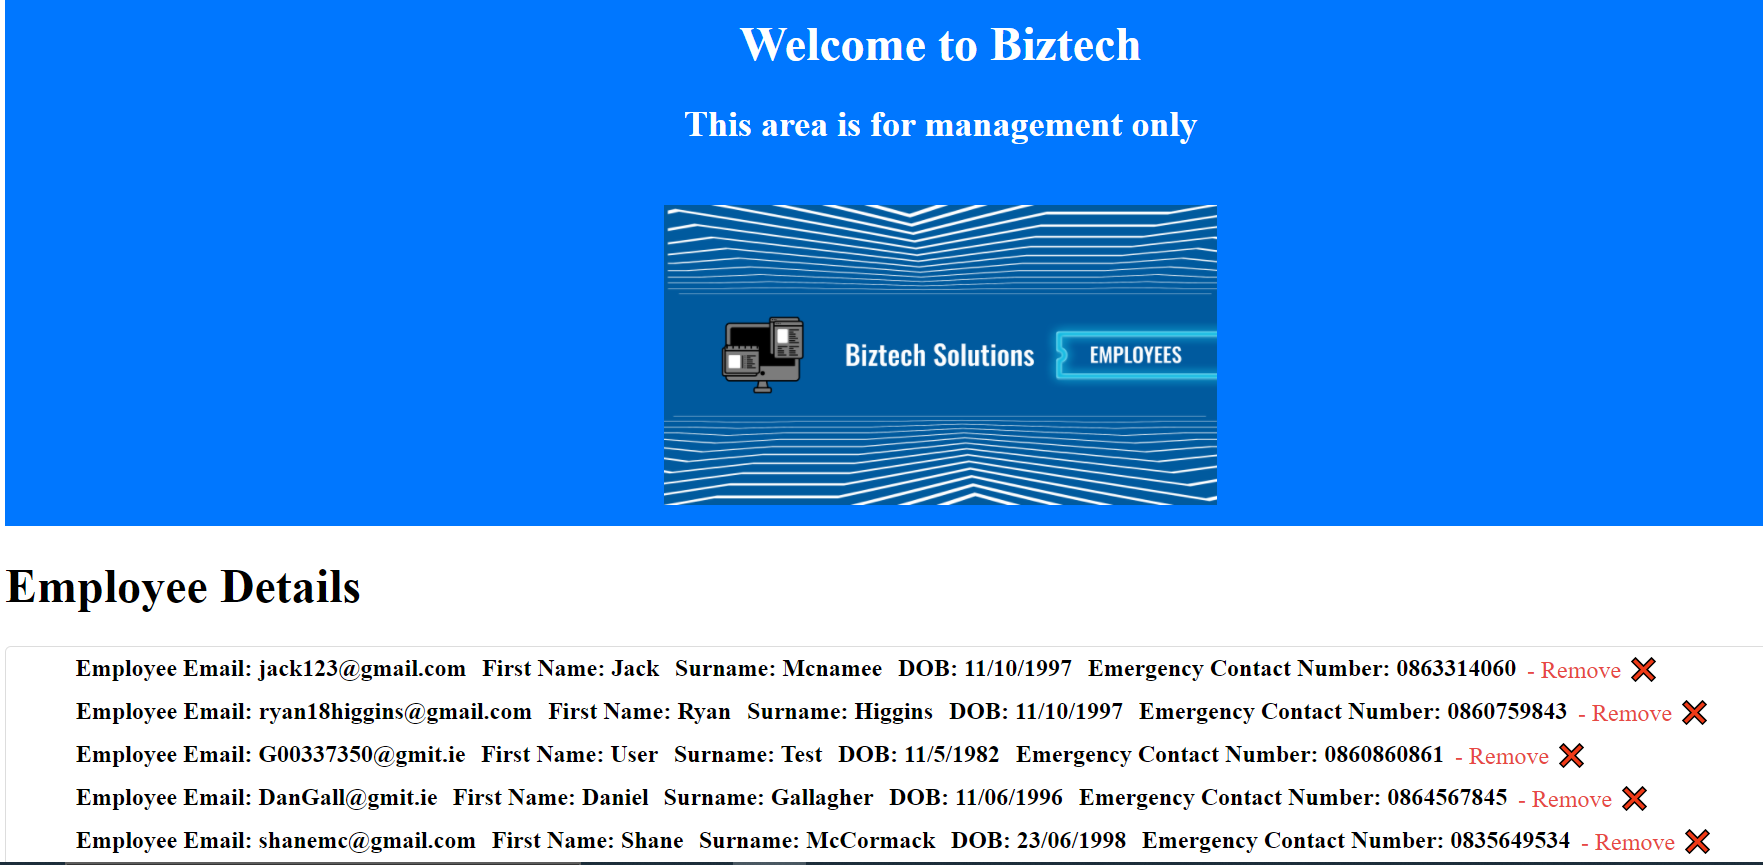
\includegraphics[scale=0.5]{img/EmployeeDetails.PNG}
    \caption{Employee Details}
    \label{fig}
\end{figure}
In the below image \textbf{(figure 5.13)} you can see the employee details side of the website. This is where a manager can quickly look to see everything about his employees from Name and Email to date of birth and emergency contacts. This is an extremely useful page for management. If an employee leaves their records can be removed also by the manager using the button on the right side. Each employee only has one record, and this can again be changed in the manager section by the manager which will update the information on the database and in turn change this information.
\FloatBarrier

\subsection{Sick Employees}
\begin{figure}[!htb]
    \centering
    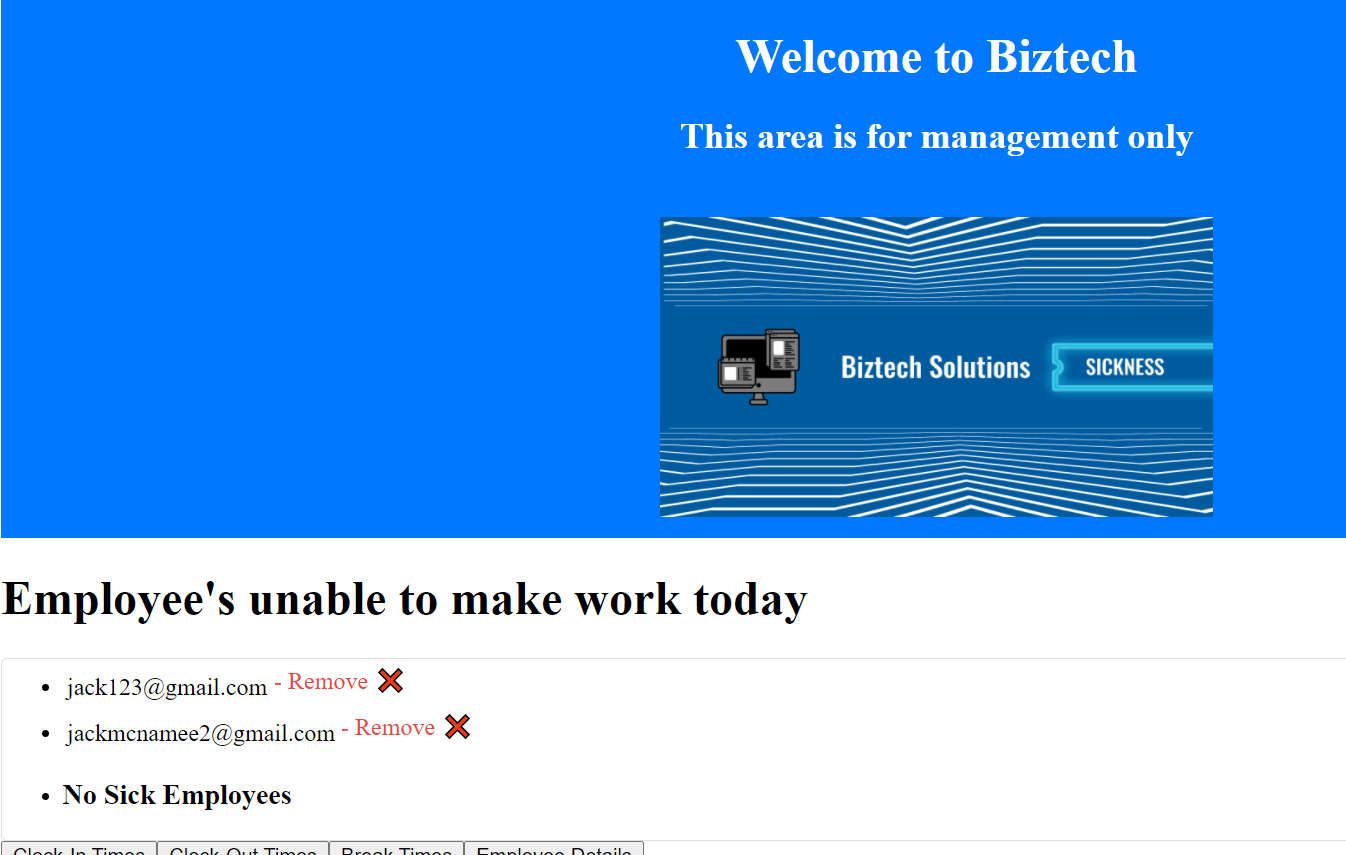
\includegraphics[scale=0.60]{img/Sickness.PNG}
    \caption{Sickness Page}
    \label{fig}
\end{figure}
In the above image \textbf{(Figure 5.14)}, for sick employees we have included a page on our website so if an employee is unable to make work due to an illness, they will be displayed here. This is done when an employees answers No to the question "Are you able to make work today?" on the application.
\FloatBarrier

\chapter{Technology Review}
\section{Testing}
When coming to the end of each sprint, we made sure to test the application constantly ourselves through the various emulators provided by Android Studio, and on physical devices. This involved testing each feature when they were completed and/or in development. For example, when we were working on the location feature, we tested the functionality by running the app in different places, physically. This allowed us to see if the geographical location of the employee, when using the app, affected the user experience and prevented the employee from clocking in, if they are not at the workplace. Then for our final sprint, we decided to do more rigorous testing, in the form of unit testing \cite{unittest} and instrumentation testing \cite{instrumentationtest}. More details on how carried out these forms of testing can be found in \hyperref[sec:Testing]{Section 6.6}.

\section{Application Performance}
We used Firebase Test Lab \cite{firebasetestlab} to do instrumentation testing on our application to see how the app performs on different devices and configurations. This also involved working with Robo Test \cite{robotest}, which imitates how a user would interact with the app. The results showed that the app ran well on multiple Android devices, with no tests failing in the process and with the layout only changing slightly depending on the smartphone. More details on instrumentation testing can be found in \hyperref[sec:Testing]{Section 6.6}.

\section{Website Performance}
We used unit testing \cite{unittest} to ensure the website is up to standard for the manager of the workplace. This involved testing the various features of the website. One such feature included displaying the employees that are unable to attend work on the sick employees page. To do so, we ensured that only the employees who answered No on the app, when answering the question: "Are you able to make work today?", would be displayed on the sick employees page. More details on testing the website can be found in \hyperref[sec:Testing]{Section 6.6}. We concluded that the website has a great user experience, is easy to follow, and has very low loading times. The website is also protected by wwwhisper \cite{wwwhisper}, a Heroku add-on, to ensure the employee details are secure, and has no negative impact to the website performance.

\section{Limitation Issues}
This app can only be released on Android devices, as the app was developed for the Android operating system. This may lead to a few employees being unable to use the application if they own an Apple smartphone. However, we found that most people own an Android smartphone, with Android having an 83.8 percent share of the smartphone market at the time of writing \cite{idc}. 
\\

We were unable to get the facial recognition feature working, which could result in other people logging into the app as an employee of the workplace. We attempted to solve this with a biometric authentication feature \cite{bioauth}, to prove that the owner of the phone that has the app is indeed an employee of the workplace, as this app would only be released to employees and the manager. However, if the device does not have the biometric authentication capability, anyone can log in to the app using the correct email and password. 
\\ 

The location feature \cite{location} could also be improved upon. This functionality involves only allowing the employee to clock in if they are at the workplace. We hoped to have the location feature working in a way that the app checks if the employee is at the workplace every few seconds and then updates the app accordingly. Unfortunately, the employee has to close the app and then reopen it to see if they can clock in. This lowers the quality of the user experience of the app and could also result in employees being late for work. 

\section{User Experience}
As this app only has one purpose, to clock in/out employees when starting/leaving work, we wanted to make it as simple and easy to use as possible. We feel that we achieved this goal as there is only functionality for what is needed, in terms of clocking in, going on break, and clocking out. This is the same for the manager side of the application, as he/she can only add employees, edit their details, and change the location of the workplace. The website also achieves this objective, as the website only consists of pages for what the manager needs, and has a login functionality to further secure the employees details. These pages include a clock in times page, a clock out times page, a break times page, an employee details page, and a sick employees page.

\chapter{Conclusion}
This chapter will summarise the project in terms of the objectives of the initial proposal that we had discussed from the start of this project
and will also discuss the findings and outcomes of the project now it has concluded.
The project proposed the development of an Android application which would be used as a Clock-In system for companies and would store the employees in a database which can only be viewed by the manager.

\section{Objectives and Goals}
\begin{itemize}
  \item Solve a problem that we have all experienced in the workplace
   \begin{center}
      \textbf{PASS}
  \end{center}
  \item Deploy an application which has facial recognition working on it for employees data protection.
   \begin{center}
      \textbf{FAIL - REPLACED WITH BIOMETRIC AUTHENTICATION}
  \end{center}
  \item Develop an application that will allow employees to clock in and out using their phone.
  \begin{center}
      \textbf{PASS}
  \end{center}
  \item Help prevent the spread and transmission of Covid-19 in the workplace.
  \begin{center}
      \textbf{PASS}
  \end{center}
  \item Design a user friendly application that will be easy to understand.
  \begin{center}
      \textbf{PASS}
  \end{center}
  \item Design a website for a manager to view the data produced by the employees when using the app.
  \begin{center}
      \textbf{PASS}
  \end{center}
  \item Ensure the app is secure and protects the employees and managers data
  \begin{center}
      \textbf{PASS}
  \end{center}
  \item To work as a team, work as professionally as possible, set objectives and complete them.
  \begin{center}
      \textbf{PASS}
  \end{center}
  \item To follow the Agile method of developing projects 
  \begin{center}
      \textbf{PASS}
  \end{center}
  \item Meet weekly with our Supervisor and team members to discuss recent updates in the project.
  \begin{center}
      \textbf{PASS}
  \end{center}
  \item Allocate the work evenly and fairly between the four of us and set goals for each one of us
  \begin{center}
      \textbf{PASS}
  \end{center}
  \item Constantly test the application which allows for error and bug detection
as well as advance the development of this application. The application should be tested every time it is updated and documented on the results.
  \begin{center}
      \textbf{PASS}
  \end{center}
\end{itemize}

\section{Retrospective of this project}
Starting off this project we had decided to take on learning a new language which was Kotlin as we believed that it was a good language to learn as we were hoping to make an android application which from our research would be done through Android studio. We had found the Kotlin, Android Studio and MongoDB documentation online extremely useful and helpful. The documentation was easy to follow and very detailed in the description of the steps necessary to complete the chosen tasks.
\\
We used the documentation in setting up the project which entailed of starting an Android application from scratch and for setting up our database but also right through the project for testing and also for deploying our application. Using MongoDB really gave us an opportunity to work on the rest of the application without having most of the back-end working. MongoDB was also included in the project for security reasons as we would be storing employees information we found it vital that security was a massive part of our project. Although we feel as a group that MongoDB worked well for our project we were not able to integrate facial recognition with MongoDB as it is not possible to use it through MongoDB so in hindsight it may have been more appropriate to use a database called Firebase. Firebase can incorporate Facial recognition which was a feature we really had hoped to had got working on our project but after many tutorials and reading lots of documentation online we had to switch to biometric authentication, as we opted to use MongoDB instead of Firebase. This was unfortunate as we had hoped to be able to prove that the employee was indeed an employee of the workplace via facial recognition.
\section{Improvements}
In this section in the conclusion we want to describe the possible improvements that we feel we could do for this project. We feel these improvements would help this application move forward in the software industry to gain popularity and improve the overall user experience while not damaging the performance of the application which is very valuable for us.
\\
\\
\textbf{Applications Improvements}
\\
There are certain aspects of the application that that did not quite come out as it was planned at the beginning and due to the project time frame certain features were not included. The improvements in the application that we believe can be made are as follows were the facial recognition feature and to develop an application for iPhone users. Due to time constraints and other elements we were unable to complete these two features. 

\chapter{Appendices}
\section{Running Application}
To run this application:

\begin{itemize}
    \item Download Android Studio. (\url{https://developer.android.com/studio}).
    \item Clone our Github repository:  
    \begin{verbatim}
    git clone https://github.com/ryanhiggins11/FINAL-YEAR-PROJECT
    \end{verbatim}
    \item Open Android Studio and select open an existing project. Search for the folder created when cloning our repository and select it. Wait for Android Studio to finish building the gradle files.
    \item Follow this tutorial to set up an emulator to run the app: 
    
    (\url{https://developer.android.com/studio/run/emulator}).
    \item Or follow this tutorial to set up a physical device to run the app: 
    
    (\url{https://developer.android.com/studio/run/device}).
    \item To sign in as an employee, use the following credentials to sign in:
    
    Email: example@biztech.com Password: example123
    \item To sign in as a manager, use the following credentials to sign in: 
    
    Email: admin@biztech.com Password: admin123
\end{itemize}


\section{Running Website}
To run the website:

\begin{itemize}
    \item Clone our Github repository:
    
    \begin{verbatim}
    git clone https://github.com/ryanhiggins11/FINAL-YEAR-PROJECT
    \end{verbatim}
    
    \item Navigate to the ManagerWebsite folder:
    \begin{verbatim}
    cd ManagerWebsite
    \end{verbatim}
    \item To install the necessary dependencies and start the server:
    
    \begin{verbatim}
    npm install
    
    npm start server
    \end{verbatim}
    \item Open a new command prompt and navigate to the client folder: 
    
    \begin{verbatim}
    cd ManagerWebsite\client
    \end{verbatim}
    \item To install necessary dependencies and run the website:
    
    \begin{verbatim}
    npm install
    
    npm start
    \end{verbatim}
\end{itemize}
